%% PREAMBLE
%% Compiler: pdfLaTeX (Overleaf default). Vietnamese quotations are wrapped in
%% \vi{...}, which switches babel to Vietnamese (T5 font encoding).
\documentclass[12pt, twoside]{report}

\usepackage[utf8]{inputenc}
\usepackage[T5,T1]{fontenc}
\usepackage[main=english,vietnamese]{babel}
\usepackage{lmodern}

\usepackage{amsmath}
\usepackage{amssymb}
\usepackage{bm}

%% \cmark for tick and \xmark for cross
\usepackage{pifont}
\newcommand{\cmark}{\ding{51}}%
\newcommand{\xmark}{\ding{55}}%

\usepackage{multirow}
\usepackage{graphicx}
\usepackage{tikz}
\usetikzlibrary{calc}

\usepackage[a4paper, top=2.5cm, bottom=2cm, left=3cm, right=2cm, bindingoffset=5mm]{geometry}
\usepackage{fancyhdr}
\usepackage{titlesec}

\usepackage{algorithm}
\usepackage{algpseudocode}
\usepackage{url}
\usepackage{listings}
\usepackage{xcolor}

\usepackage{booktabs}
\usepackage{tabularx}
\usepackage{array}
\usepackage{float}
\usepackage{caption}
\usepackage{enumitem}
\usepackage{setspace}
\onehalfspacing
%% Let long code paths (\texttt) break and give paragraphs extra stretch,
%% which removes most Overfull \hbox warnings without visible loosening.
\usepackage[htt]{hyphenat}
\setlength{\emergencystretch}{2em}
\setlist{itemsep=2pt, topsep=4pt}
\captionsetup{font=small, labelfont=bf}
\newcolumntype{L}{>{\raggedright\arraybackslash}X}

%% Python listings
\lstdefinestyle{mystyle}{
	basicstyle=\ttfamily\footnotesize,
	breakatwhitespace=false,
	breaklines=true,
	captionpos=b,
	frame=single,
	keepspaces=true,
	numbers=left,
	numbersep=5pt,
	numberstyle=\tiny\color{black},
	showstringspaces=false,
	keywordstyle=\color{blue}\bfseries,
	commentstyle=\color{gray}\itshape,
	stringstyle=\color{teal},
	columns=fullflexible,
	upquote=true,
	literate={—}{{---}}1 {–}{{--}}1 {→}{{$\rightarrow$}}1 {≥}{{$\geq$}}1,
}
\lstset{style=mystyle}

%% Customize chapter titles
\titleformat{\chapter}[display]
  {\Huge\bfseries\centering}{\chaptername~\thechapter}
  {0pt}
  {\Huge}
\titlespacing*{\chapter}
  {0pt}
  {*0}
  {1em}

%% Fix appendix labeling
\makeatletter
\newcommand\AppendixName{Appendix}
\let\oldappendix\appendix
\renewcommand{\appendix}{%
  \oldappendix
  \renewcommand{\chaptername}{\AppendixName}  \renewcommand{\thechapter}{\@Alph\c@chapter}}
\makeatother
\addto\captionsenglish{\renewcommand*\contentsname{Table of Contents}}
\addto{\extrasenglish}{%
  \renewcommand{\bibname}{References}
}
\renewcommand\lstlistlistingname{List of Listings}

%% All figure files live in images/
\graphicspath{{images/}}

%% ---------------------------------------------------------------------------
%% Project macros
%% ---------------------------------------------------------------------------
%% Vietnamese inline text (switches hyphenation and font encoding).
\newcommand{\vi}[1]{\foreignlanguage{vietnamese}{#1}}
%% Code identifiers.
\newcommand{\code}[1]{\texttt{#1}}

%% \diagram{file}{width}{caption}{label}
%% Includes images/<file> when it exists; otherwise draws a framed placeholder
%% so the report still compiles before the Mermaid diagrams are exported
%% (see report/REPORT_DIAGRAMS.md).
\newcommand{\diagram}[4]{%
	\begin{figure}[htbp]
		\centering
		\IfFileExists{images/#1}{%
			\includegraphics[width=#2\linewidth,height=0.7\textheight,keepaspectratio]{#1}%
		}{%
			\fbox{\parbox[c][5cm][c]{0.9\linewidth}{\centering\large\ttfamily
				Insert diagram: images/\detokenize{#1}\\[4pt]
				\normalsize (Mermaid source in report/REPORT\_DIAGRAMS.md)}}%
		}
		\caption{#3}
		\label{#4}
	\end{figure}%
}


%% \screenshot{file}{width}{caption}{label}: same idea as \diagram, for UI captures.
\newcommand{\screenshot}[4]{%
	\begin{figure}[htbp]
		\centering
		\IfFileExists{images/#1}{%
			\fbox{\includegraphics[width=#2\linewidth,height=0.6\textheight,keepaspectratio]{#1}}%
		}{%
			\fbox{\parbox[c][5cm][c]{0.9\linewidth}{\centering\large\ttfamily
				Insert screenshot: images/\detokenize{#1}}}%
		}
		\caption{#3}
		\label{#4}
	\end{figure}%
}

\usepackage[hidelinks]{hyperref}
\hypersetup{
	pdftitle={An LLM-Powered Application for Detecting Academic Stress Levels in Vietnamese University Students},
	pdfauthor={Nguyen Minh Tuan (ITCSIU22298)},
	pdfsubject={Pre-thesis, School of Computer Science and Engineering, International University - VNU-HCM},
}

\begin{document}
\pagenumbering{roman}

\newgeometry{top=2.5cm, bottom=2.5cm, left=2.5cm, right=2.5cm}

%% Title page
\begin{titlepage}

	\begin{tikzpicture}[remember picture,overlay,inner sep=0,outer sep=0]
     %% Frame corners, measured from the physical page.
     \coordinate (NW) at ([xshift=1.5cm,yshift=-2cm]current page.north west);
     \coordinate (SE) at ([xshift=-1.5cm,yshift=2cm]current page.south east);
     %% Thick blue frame.
     \draw[blue!70!black,line width=4pt] (NW) rectangle (SE);
     %% Thin crossing frames at 0.5cm and 0.3cm: one inset horizontally and outset
     %% vertically, the other the reverse, which forms the corner squares.
     %% (Replaces the template's chained path, whose D-to-A segment had a sign
     %% typo and drew a stray diagonal line down the right-hand side.)
     \foreach \d in {0.5cm,0.3cm} {
       \draw ([xshift=\d,yshift=\d]NW) rectangle ([xshift=-\d,yshift=-\d]SE);
       \draw ([xshift=-\d,yshift=-\d]NW) rectangle ([xshift=\d,yshift=\d]SE);
     }

   \end{tikzpicture}

	\centering
	\textbf{VIETNAM NATIONAL UNIVERSITY HO CHI MINH CITY}\par \textbf{THE
		INTERNATIONAL UNIVERSITY}\par \textbf{SCHOOL OF COMPUTER SCIENCE AND ENGINEERING}\par

	\vspace{1.5cm}
	
\includegraphics[width=0.25\textwidth]{IU.png}

	\vspace{1cm}
	{\large\textbf{AN LLM-POWERED APPLICATION FOR DETECTING ACADEMIC STRESS LEVELS IN VIETNAMESE UNIVERSITY STUDENTS}}

	\vspace{1cm}
	By \par \textbf{NGUYEN MINH TUAN}\par Student ID: ITCSIU22298

	\vspace{1cm}
	Supervisor: \textbf{Dr.~Ho Long Van}

	\vspace{1.5cm}
	\textit{A pre-thesis submitted to the School of Computer Science and Engineering \\ in partial
		fulfillment of the requirements for the degree of \\ Bachelor of Engineering in Computer Science}

	\vspace{1.5cm}
	\text{Ho Chi Minh City, Vietnam} \par September 2026

	\newpage

	%% Signature page
	\centering

	{\large\textbf{AN LLM-POWERED APPLICATION FOR DETECTING ACADEMIC STRESS LEVELS IN VIETNAMESE UNIVERSITY STUDENTS}}\par
	\vspace{3cm}

	\hspace{7cm}
	\makebox[7cm][l]{\text{APPROVED BY:}}
	\par
	\vspace{2cm}

	\hspace{7cm}
	\makebox[7cm][l]{\underline{\hspace{7cm}}}
	\par \hspace{7cm}
	\makebox[7cm][l]{\textit{Dr.~Ho Long Van, Supervisor}}
	\par
	\vspace{2cm}

	\hspace{7cm}
	\makebox[7cm][l]{\underline{\hspace{7cm}}}
	\par \hspace{7cm}
	\makebox[7cm][l]{\textit{[Committee member]}}
	\par
	\vspace{2cm}

	\hspace{7cm}
	\makebox[7cm][l]{\underline{\hspace{7cm}}}
	\par \hspace{7cm}
	\makebox[7cm][l]{\textit{[Committee member]}}
	\par
	\vspace{2cm}

	\hspace{7cm}
	\makebox[7cm][l]{\underline{\hspace{7cm}}}
	\par \hspace{7cm}
	\makebox[7cm][l]{\textit{[Committee member]}}
	\par
	\vspace{0.75cm}

	\hspace{7cm}
	\makebox[7cm][r]{\text{THESIS COMMITTEE}}
	\par
	\thispagestyle{empty}
\end{titlepage}
\restoregeometry

%% Acknowledgments
\chapter*{Acknowledgments}
I would like to express my sincere gratitude to my supervisor, Dr.~Ho Long Van, for the guidance, critical questions and encouragement given throughout this pre-thesis. I also thank the School of Computer Science and Engineering, International University --- Vietnam National University Ho Chi Minh City, for the knowledge and resources that made this work possible.

Finally, I thank my family and friends for their patience and support during the months spent building and evaluating this system.
\thispagestyle{empty}

%% Table of Contents, List of Figures, List of Tables
\tableofcontents
\listoftables
\addcontentsline{toc}{chapter}{List of Tables}
\listoffigures
\addcontentsline{toc}{chapter}{List of Figures}
\listofalgorithms
\addcontentsline{toc}{chapter}{List of Algorithms}
\lstlistoflistings
\addcontentsline{toc}{chapter}{List of Listings}

%% Abstract
\chapter*{Abstract}
\addcontentsline{toc}{chapter}{Abstract}
Academic stress is a persistent concern among Vietnamese university students, yet help-seeking remains low and counselling capacity is limited. This pre-thesis presents the design, implementation and preliminary evaluation of a web application that estimates a student's academic stress level from free text and two validated psychometric instruments, and returns coping suggestions grounded in a curated knowledge base. The system combines deterministic scoring of the DASS-21 and PSS-10, a PhoBERT classifier fine-tuned for Vietnamese stress classification, and a retrieval-augmented large language model (LLM) that writes an explanation and three actionable suggestions with verified citations. A deterministic crisis-detection gate runs before any data is stored and before any LLM call; when it fires, the assessment is replaced by mental-health helpline information and nothing the student wrote is persisted.

Six systems were compared on one frozen, stratified 70-item test split in a unified four-class label space. TF-IDF with logistic regression reached accuracy 0.686 and macro-F1 0.682; fine-tuned PhoBERT 0.657 and 0.533; zero-shot LLM prompting 0.529 and 0.524; and the full proposed pipeline 0.486 and 0.500. An ablation shows that removing the questionnaire scores collapses the pipeline to the majority-class floor (macro-F1 0.123), so its agreement with the questionnaire-derived label is largely circular. Retrieval quality over a 57-query labelled set gave MRR 0.787 and Recall@5 0.903, and a paired comparison exposed a defect in the deployed query construction; rewriting it raised MRR on the affected queries from 0.509 to 0.839. The crisis rule was rebuilt around six constructs from suicide-risk assessment and measured on a 60-item bilingual set frozen before the patterns were written: precision rose from 0.600 to 1.000 and recall from 0.200 to 0.867, with no false positives on twenty lethal-sounding idioms. The principal limitation is the data: every classification figure was computed on text generated from 41 Vietnamese sentence templates, and 34 of 70 test items are more than 0.80 similar to a training item. These figures therefore demonstrate the pipeline rather than real-world stress detection. Infrastructure for a consented real-data study is implemented but has not yet been run. The system screens and estimates; it does not diagnose.

\vspace{0.5em}
\noindent\textbf{Keywords:} academic stress, Vietnamese NLP, PhoBERT, retrieval-augmented generation, DASS-21, PSS-10, crisis detection, mental-health screening

%% Chapters
\chapter{INTRODUCTION}\label{ch:intro}
\pagenumbering{arabic}
\setcounter{page}{1}
This chapter motivates the work, states the problem precisely, defines what is and is not in scope, and sets five measurable objectives against which Chapter~\ref{ch:conclusion} judges the outcome.

\section{Motivation}
Academic stress among university students is a widely documented concern, and its severity is shaped by the educational culture in which it occurs. In Vietnam, academic achievement is closely tied to family expectation and social standing, examination competition is intense, and the transition into university often coincides with relocation, financial independence and the loss of established support networks. These pressures are compounded for students in high-workload disciplines and for those who study far from their home province. Epidemiological studies of stress, anxiety and depression among Vietnamese university students exist; this report deliberately quotes no prevalence figure, because no source for one was verified within the scope of this work. The motivation rests instead on two structural factors that can be stated without a contested number.

The first is the \textbf{help-seeking gap}. Mental-health stigma remains substantial, and students frequently interpret psychological distress as a personal failing rather than a health condition. Walking into a counselling office is a visible, socially costly signal, so the students who most need support are often the least likely to ask for it. The second is \textbf{capacity}: even where students are willing to seek help, the ratio of counsellors to enrolled students makes routine screening infeasible by human effort alone.

A private, self-administered digital screening tool addresses both factors at once. It removes the visibility cost of the first contact and scales without consuming counsellor time. It does not replace clinical judgment; its function is to help a student notice a pattern in their own experience and, where appropriate, to lower the barrier to the next step.

Building such a tool for Vietnamese students raises technical problems that are not solved by transferring an English-language system. Vietnamese diacritics carry both phonemic and tonal information, so their routine omission in informal writing is genuinely ambiguating: \vi{ma, má, mà, mả, mã, mạ} are six distinct words. Vietnamese is an isolating language in which a syllable is not a word - \vi{áp lực} (``pressure'') is two syllables and one lexical item - so whitespace tokenisation fragments meaning. Student writing adds \textit{teencode}, code-switching with English academic vocabulary, and register shifts driven by the pronoun system. Most consequentially for a supervised approach, \textbf{no public annotated Vietnamese corpus of student mental-health text exists}.

\section{Problem Statement}
Given a university student's free-text description of their recent experience, optional responses to validated psychometric instruments, and optional information about their academic and personal circumstances, the system must produce:

\begin{enumerate}
	\item an \textbf{estimated academic-stress level} on an interpretable ordinal scale (Low, Moderate, High, Severe);
	\item an \textbf{explanation} identifying which evidence drove the estimate; and
	\item \textbf{actionable coping suggestions} appropriate to that student's circumstances and grounded in vetted material,
\end{enumerate}

\noindent while \textit{never} producing a clinical diagnosis, and while reliably diverting students who disclose self-harm risk to human support instead of an automated assessment.

Four aspects of this problem are not solved by existing work. First, the instruments used for stress screening are validated as self-report questionnaires, not as targets for text-based prediction. Second, text-based mental-health detection is overwhelmingly English-language and trained on public social-media posts, whose register differs from a private self-report. Third, LLM-generated advice carries a well-documented hallucination risk~\cite{ji2023hallucination} that is unacceptable in a mental-health context, and its standard mitigation, retrieval grounding~\cite{lewis2020rag}, is rarely evaluated as a component in its own right. Fourth, the safety layer that such systems require is frequently asserted but rarely measured.

\section{Scope}
This pre-thesis covers the design, implementation and preliminary evaluation of the system described above. The scope is bounded as follows:

\begin{enumerate}
	\item \textbf{In scope.}
	      \begin{itemize}
	      	\item A working web application: a \textbf{Streamlit} interface over a \textbf{FastAPI} backend, with consent, questionnaires, free text, context, results and history.
	      	\item \textbf{Deterministic scoring} of the DASS-21~\cite{lovibond1995} and PSS-10~\cite{cohen1983} exactly as published.
	      	\item A \textbf{PhoBERT} classifier~\cite{nguyen2020phobert} fine-tuned on Vietnamese student text.
	      	\item A \textbf{retrieval-augmented} advisory module over a curated knowledge base, with citation verification.
	      	\item A \textbf{crisis-detection gate} and its quantitative evaluation on labelled test sets.
	      	\item A \textbf{reproducible evaluation harness} comparing baselines, the fine-tuned classifier and LLM systems on one frozen split.
	      \end{itemize}
	\item \textbf{Out of scope.}
	      \begin{itemize}
	      	\item \textit{Clinical validation} or any claim of diagnostic accuracy.
	      	\item \textit{Deployment to a live student population} and longitudinal tracking.
	      	\item \textit{Collection of real participant data}: the collection pipeline is implemented and verified, but no participant has contributed data.
	      \end{itemize}
\end{enumerate}

\section{Objectives}
Five measurable objectives are defined, each tied to an experiment in Chapter~\ref{ch:result}.

\begin{description}[style=nextline, leftmargin=1.2cm]
	\item[O1 - Psychometric scoring.] Implement DASS-21 and PSS-10 exactly per their published scoring rules, with deterministic, testable behaviour. \textit{Measured by} unit tests against hand-computed fixtures including all-zero, all-maximum and reverse-scored cases.
	\item[O2 - Text classification.] Fine-tune a Vietnamese pre-trained encoder for stress classification and compare it with classical and generative baselines on one identical held-out split. \textit{Measured by} accuracy, macro-F1, Cohen's $\kappa$ and per-class F1 on the same 70-item test set.
	\item[O3 - Grounded advice.] Build a retrieval-augmented advisory module over a curated knowledge base and evaluate each component's contribution. \textit{Measured by} retrieval metrics over a labelled query set and a component ablation.
	\item[O4 - Safety.] Implement a crisis-detection gate and evaluate it quantitatively. \textit{Measured by} precision, recall and F1 on a held-out labelled set, with per-category breakdown and verbatim errors.
	\item[O5 - Reproducibility.] Build an evaluation infrastructure in which no reported number exists without a script that produced it. \textit{Measured by} traceability of every figure to a versioned artefact and explicit ``not run'' markers for missing measurements.
\end{description}

\section{Contributions}
\begin{enumerate}
	\item \textbf{An end-to-end, working screening application} integrating validated psychometric scoring, a fine-tuned Vietnamese transformer, retrieval-augmented generation with verified citations, and a pre-persistence, pre-generative safety gate.
	\item \textbf{A construct-based bilingual crisis-detection rule} with an evaluation procedure designed to avoid tuning on the test set: the held-out set was written and frozen before the patterns existed.
	\item \textbf{A measured correction to the retrieval pipeline}: a paired query-construction experiment located a defect that halved retrieval effectiveness on affected queries, and the fix was chosen by measurement.
	\item \textbf{A leakage characterisation for template-generated data}, showing that exact-duplicate checks - the usual control - give no protection when test items are near-copies of training items.
	\item \textbf{A reproducible evaluation harness} with frozen splits, content-addressed LLM caching and explicit ``not run'' markers in place of estimates.
\end{enumerate}

\section{Structure of the Report}
Chapter~2 reviews related work and the theory the system relies on. Chapter~3 states the requirements, use cases and algorithms. Chapter~4 presents the architecture and the design strategies behind it. Chapter~5 describes the implementation. Chapter~6 reports the prototype and every experimental result. Chapter~7 interprets the results, including strengths, limitations and comparison with related work. Chapter~8 concludes against the five objectives. The appendices contain code listings, instrument items, prompts, crisis-rule errors and reproducibility commands.


\chapter{RELATED WORK}\label{ch:work}
This chapter reviews the literature this work builds on: stress instruments, text-based mental-health detection, Vietnamese language models, and LLMs with retrieval augmentation. It then identifies the research gap and summarises the theory used in later chapters.

\section{Current Advancements}

\subsection{Psychometric instruments for stress}
Psychological stress is conventionally modelled as a perceived imbalance between environmental demand and appraised capacity to cope. Two self-report instruments dominate applied screening and are both used here. The \textbf{Depression Anxiety Stress Scales, 21-item version (DASS-21)}~\cite{lovibond1995} measures three related negative emotional states; its stress subscale targets persistent arousal, difficulty relaxing, irritability and over-reactivity. The \textbf{Perceived Stress Scale (PSS-10)}~\cite{cohen1983} measures how unpredictable, uncontrollable and overloading life is appraised to be; normative data were later published by Cohen and Williamson~\cite{cohen1988}. Cohen did not publish clinical cut-offs for the PSS-10; the common 0--13 / 14--26 / 27--40 bands are a convention, and this report treats them as such. A Vietnamese DASS-21 has been validated in a community sample~\cite{tran2013}.

\subsection{Machine learning for mental-health detection from text}
Automated detection of psychological state from text has developed in three overlapping phases. \textit{Classical feature engineering} combined lexicons, n-grams and pronoun usage with linear classifiers; these remain strong baselines because they are interpretable and need little data. \textit{Neural sequence models} improved on n-grams where large labelled sets existed. \textit{Transfer learning from pre-trained transformers}~\cite{devlin2019} changed the field by making competitive performance possible from hundreds rather than tens of thousands of labelled examples - the regime of this work.

The datasets that shaped the field are English. The CLPsych 2015 shared task~\cite{coppersmith2015} evaluated depression and PTSD signals on Twitter; \textbf{Dreaddit}~\cite{turcan2019} annotated Reddit posts for stress and is the closest analogue to this task; the eRisk collection~\cite{losada2016} introduced early risk detection over sequences of posts. All are valuable methodological references, but none is directly usable here: the language differs, and so does the register - a public social-media post is a performance, a private self-report to a screening tool is not.

\subsection{Vietnamese natural language processing}
\textbf{PhoBERT}~\cite{nguyen2020phobert} is a RoBERTa-style encoder pre-trained on 20\,GB of Vietnamese text and is the standard encoder for Vietnamese classification. It was pre-trained on \textit{word-segmented} text, produced by \textbf{VnCoreNLP}~\cite{vu2018vncorenlp}, so unsegmented input differs from its pre-training distribution. \textbf{XLM-RoBERTa}~\cite{conneau2020xlmr} is a multilingual alternative covering 100 languages, and \textbf{ViSoBERT}~\cite{nguyen2023visobert} targets Vietnamese social-media text, including teencode. For semantic retrieval, \textbf{Sentence-BERT}~\cite{reimers2019sbert} introduced efficient bi-encoder sentence embeddings, and multilingual knowledge distillation~\cite{reimers2020multilingual} produced the multilingual encoder used by this system's retriever.

\subsection{Large language models and retrieval-augmented generation}
Large language models~\cite{brown2020gpt3} follow instructions and classify zero-shot, which is attractive when labelled data is scarce. They also generate fluent, confident, false statements; Ji et al.~\cite{ji2023hallucination} distinguish \textit{intrinsic} hallucination, which contradicts the source, from \textit{extrinsic} hallucination, which cannot be verified from it. \textbf{Retrieval-augmented generation (RAG)}~\cite{lewis2020rag} conditions generation on passages retrieved from a controlled corpus, constraining assertions and enabling attribution. That benefit holds only if retrieval returns relevant passages, the model actually uses them, and the system behaves safely when retrieval returns nothing - three conditions that are often assumed rather than measured. In mental-health applications the operative safety properties are not fluency or empathy but reliable escalation on risk disclosure, refusal to diagnose, and avoidance of advice that substitutes for professional care.

\subsection{Usability and human evaluation}
For future human evaluation this work adopts established instruments: Krippendorff's $\alpha$~\cite{krippendorff2004} for inter-rater agreement, the System Usability Scale~\cite{brooke1996sus}, and Bangor et al.'s adjective bands for interpreting SUS scores~\cite{bangor2009sus}.

\section{Research Gap}
Table~\ref{tab:gap} positions representative work against the capabilities this project combines.

\begin{table}[ht]
	\centering
	\caption{Capabilities of representative related work (\protect\cmark: yes, \protect\xmark: no).}
	\label{tab:gap}
	\resizebox{\textwidth}{!}{%
		\begin{tabular}{lcccccc}
			\toprule
			                                   & \textbf{This work} & Dreaddit~\cite{turcan2019} & CLPsych~\cite{coppersmith2015} & eRisk~\cite{losada2016} & PhoBERT~\cite{nguyen2020phobert} & RAG~\cite{lewis2020rag} \\ \midrule
			Vietnamese text                    & \cmark             & \xmark                     & \xmark                         & \xmark                  & \cmark                           & \xmark                  \\
			Mental-health / stress target      & \cmark             & \cmark                     & \cmark                         & \cmark                  & \xmark                           & \xmark                  \\
			Validated questionnaire scoring    & \cmark             & \xmark                     & \xmark                         & \xmark                  & \xmark                           & \xmark                  \\
			Retrieval-grounded generation      & \cmark             & \xmark                     & \xmark                         & \xmark                  & \xmark                           & \cmark                  \\
			Measured crisis / safety layer     & \cmark             & \xmark                     & \xmark                         & \xmark                  & \xmark                           & \xmark                  \\
			Human-annotated real data          & \xmark             & \cmark                     & \cmark                         & \cmark                  & \cmark                           & \cmark                  \\ \bottomrule
		\end{tabular}%
	}
\end{table}

The literature therefore provides: validated stress instruments without a text modality; English detection systems trained on a public register that differs from private self-report; Vietnamese encoders without a mental-health corpus to fine-tune on; and a retrieval architecture whose safety benefit is widely assumed but seldom measured. No published work known to the author combines validated psychometric scoring, Vietnamese text classification and retrieval-grounded advice in one evaluated system for Vietnamese university students, or reports a quantitative evaluation of a Vietnamese crisis-detection layer. This work addresses that combination. The last row of Table~\ref{tab:gap} is its weakest point: it has no real, human-annotated data yet, which Chapter~\ref{ch:discussion} treats as the binding limitation.

\section{Theoretical Background}

\subsection{Psychometric scoring}
\label{sec:theory-scoring}
\subsubsection{DASS-21}
Let $A=\{a_1,\dots,a_{21}\}$ with $a_i\in\{0,1,2,3\}$, and let $I_d, I_a, I_s$ be the seven item indices of the depression, anxiety and stress subscales. Each subscale score is doubled to stay comparable with the 42-item DASS~\cite{lovibond1995}:
\begin{align}
	S_k = 2\sum_{i\in I_k} a_i, \qquad k\in\{d,a,s\}. \label{eq:dass}
\end{align}
Each $S_k$ is mapped to a severity band using the cut-offs in Table~\ref{tab:dass-cutoffs}.

\begin{table}[ht]
	\centering
	\caption[DASS-21 subscale items and severity cut-offs]{DASS-21 subscale items and severity cut-offs (applied to doubled scores)~\cite{lovibond1995}.}
	\label{tab:dass-cutoffs}
	\resizebox{\textwidth}{!}{%
		\begin{tabular}{llccccc}
			\toprule
			Subscale   & Items                   & Normal & Mild  & Moderate & Severe & Extremely severe \\ \midrule
			Depression & 3, 5, 10, 13, 16, 17, 21 & 0--9   & 10--13 & 14--20   & 21--27 & $\geq 28$        \\
			Anxiety    & 2, 4, 7, 9, 15, 19, 20   & 0--7   & 8--9  & 10--14   & 15--19 & $\geq 20$        \\
			Stress     & 1, 6, 8, 11, 12, 14, 18  & 0--14  & 15--18 & 19--25   & 26--33 & $\geq 34$        \\ \bottomrule
		\end{tabular}%
	}
\end{table}

\subsubsection{PSS-10}
Let $R=\{r_1,\dots,r_{10}\}$ with $r_j\in\{0,\dots,4\}$ and $J=\{4,5,7,8\}$ the positively worded, reverse-scored items. Then
\begin{align}
	P = \sum_{j\notin J} r_j + \sum_{j\in J}(4-r_j), \qquad P\in[0,40], \label{eq:pss}
\end{align}
categorised as Low (0--13), Moderate (14--26) or High (27--40).

\subsection{Transformer fine-tuning}
PhoBERT-base is a 12-layer encoder (hidden size 768, 12 attention heads). For classification, a dense layer with $\tanh$ activation is applied to the first-token representation, followed by a linear projection to $C$ logits $z_{n,c}$. Training minimises class-weighted cross-entropy to counter label imbalance:
\begin{align}
	\mathcal{L} = -\frac{1}{N}\sum_{n=1}^{N} w_{y_n}\log\frac{\exp(z_{n,y_n})}{\sum_{c=1}^{C}\exp(z_{n,c})}, \qquad w_c=\frac{N}{C\cdot N_c}, \label{eq:loss}
\end{align}
where $N_c$ is the number of training examples in class $c$. Parameters are updated with AdamW, which decouples weight decay $\lambda$ from the adaptive step:
\begin{align}
	m_t &= \beta_1 m_{t-1} + (1-\beta_1)g_t, \qquad v_t = \beta_2 v_{t-1} + (1-\beta_2)g_t^2, \\
	\vartheta_t &= \vartheta_{t-1} - \eta_t\left(\frac{\hat m_t}{\sqrt{\hat v_t}+\epsilon} + \lambda\vartheta_{t-1}\right), \qquad \hat m_t=\frac{m_t}{1-\beta_1^t},\ \hat v_t=\frac{v_t}{1-\beta_2^t}.
\end{align}

\subsection{Dense retrieval}
A bi-encoder $f$ maps a query $q$ and each knowledge chunk $d$ to vectors, and chunks are ranked by cosine similarity
\begin{align}
	\mathrm{sim}(q,d) = \frac{f(q)\cdot f(d)}{\lVert f(q)\rVert\,\lVert f(d)\rVert}. \label{eq:cos}
\end{align}
The top-$k$ chunks are inserted into the LLM prompt. An approximate nearest-neighbour index (HNSW) makes the search sub-linear.

\subsection{Evaluation metrics}
\label{sec:metrics}
\subsubsection{Classification}
For per-class precision $P_c$ and recall $R_c$,
\begin{align}
	F1_c = \frac{2P_cR_c}{P_c+R_c}, \qquad \text{macro-F1} = \frac{1}{C}\sum_{c=1}^{C}F1_c. \label{eq:f1}
\end{align}
Macro-F1 is the primary metric because the labels are imbalanced and the minority class (Severe) is the most consequential. Chance-corrected agreement is reported as Cohen's $\kappa=(p_o-p_e)/(1-p_e)$, where $p_o$ is observed agreement and $p_e$ agreement expected from the marginals.

\subsubsection{Retrieval}
For a query with relevant set $G$ and ranked results $r_1, r_2, \dots$:
\begin{align}
	\text{Recall@}k &= \frac{|\{r_1,\dots,r_k\}\cap G|}{|G|}, \qquad
	\text{MRR} = \frac{1}{|Q|}\sum_{q\in Q}\frac{1}{\mathrm{rank}_q}, \\
	\text{nDCG@}k &= \frac{\sum_{i=1}^{k} \mathrm{rel}_i/\log_2(i+1)}{\sum_{i=1}^{\min(k,|G|)} 1/\log_2(i+1)},
\end{align}
where $\mathrm{rank}_q$ is the position of the first relevant chunk and $\mathrm{rel}_i\in\{0,1\}$.

\subsubsection{Sampling uncertainty}
For an accuracy estimate $\hat p$ on $n$ items, the 95\,\% Wilson interval half-width is bounded, in the worst case $\hat p=0.5$, by approximately $1.96\sqrt{0.25/n}$. At $n=40$ this is $\pm0.148$ (the ablation noise floor used in Section~\ref{sec:res-ablation}); at $n=70$ it is $\pm0.113$.


\chapter{METHODOLOGY}\label{ch:method}
This chapter specifies what the system must do and how it decides. It first analyses the requirements, use cases and overall data flow, then formalises the four algorithms at the core of the system - label derivation, the assessment pipeline, crisis detection and grounded retrieval - and finally defines the evaluation design used in Chapter~\ref{ch:result}.

\section{Requirement Analysis}
Requirements were derived from the problem statement (Section~1.2), from the ethical obligations of a mental-health screening tool, and from the consent instrument written for the planned real-data study.

\begin{table}[ht]
	\centering
	\caption{Functional requirements.}
	\label{tab:fr}
	\begin{tabularx}{\textwidth}{lL}
		\toprule
		ID   & Requirement \\ \midrule
		FR1  & The student must give informed consent before any other page or data entry is available. \\
		FR2  & The student can write a free-text reflection in Vietnamese or English. \\
		FR3  & The student can complete the DASS-21 and PSS-10 with their published response anchors. \\
		FR4  & The student can optionally provide academic, lifestyle and coping context. \\
		FR5  & The system scores both instruments exactly as published and derives a four-level stress label. \\
		FR6  & The system analyses the free text (stress keywords; PhoBERT stress level for Vietnamese input). \\
		FR7  & The system checks for crisis signals and, if found, shows helplines instead of an assessment. \\
		FR8  & The system retrieves relevant knowledge-base passages and generates an explanation and up to three suggestions citing them. \\
		FR9  & The student can view their assessment history and trend. \\
		FR10 & The student can permanently delete all of their stored data. \\
		FR11 & A researcher can export an anonymised dataset and run the evaluation harness from the command line. \\ \bottomrule
	\end{tabularx}
\end{table}

\begin{table}[ht]
	\centering
	\caption{Non-functional requirements.}
	\label{tab:nfr}
	\begin{tabularx}{\textwidth}{lL}
		\toprule
		ID   & Requirement \\ \midrule
		NFR1 & \textbf{Safety.} The crisis check runs before any persistence and before any external call; a crisis disclosure is never stored. \\
		NFR2 & \textbf{Non-diagnosis.} No output may name a disorder; every response carries a non-diagnostic disclaimer. \\
		NFR3 & \textbf{Graceful degradation.} If the classifier, retriever or LLM fails, deterministic scores are still returned with a stated reason. \\
		NFR4 & \textbf{Grounding.} Advice may only come from retrieved material; citations not in the retrieved set are discarded. \\
		NFR5 & \textbf{Privacy.} Identity is a random UUID; no name, student number, e-mail or phone is collected or sent to the LLM. \\
		NFR6 & \textbf{Latency.} The deterministic path (scoring, crisis rule, lexicon, retrieval, classifier) completes in well under one second on CPU. \\
		NFR7 & \textbf{Reproducibility.} Every reported number is produced by a script on a frozen split; LLM calls are cached by input hash. \\
		NFR8 & \textbf{Maintainability.} Automated tests and linting run in continuous integration on every push. \\ \bottomrule
	\end{tabularx}
\end{table}

\subsection{Use Case Description}
Three actors interact with the system: the \textbf{Student} (primary user), the \textbf{Researcher} (command-line access to exports and evaluation), and the \textbf{LLM provider} (an external system that generates explanations). Table~\ref{tab:uc-main} describes the central use case in detail; Table~\ref{tab:uc-other} summarises the others.

\begin{table}[ht]
	\centering
	\caption{Use case UC6 - Receive stress assessment.}
	\label{tab:uc-main}
	\begin{tabularx}{\textwidth}{lL}
		\toprule
		Field          & Description \\ \midrule
		Actors         & Student (primary), LLM provider (secondary) \\
		Preconditions  & Consent given (UC1); at least free text or one questionnaire submitted. \\
		Main flow      & 1.~Student opens the Results page. 2.~System analyses the text and scores the questionnaires. 3.~System runs the crisis check. 4.~System stores the inputs. 5.~System retrieves four knowledge passages. 6.~System asks the LLM for an explanation and suggestions. 7.~System verifies the citations. 8.~System shows the questionnaire-derived level as the headline, with the explanation, suggestions and sources. \\
		Alternative A1 & At step 3 a crisis signal is found: the system shows helplines only; nothing is stored; steps 4--8 are skipped (UC7). \\
		Alternative A2 & At step 5 nothing is retrieved: the LLM is not called; scores are shown with the reason advice was withheld. \\
		Alternative A3 & At step 6 the LLM fails: scores are shown with a message that suggestions are temporarily unavailable. \\
		Postconditions & A prediction row is stored (except in A1); the assessment appears in History. \\ \bottomrule
	\end{tabularx}
\end{table}

\begin{table}[ht]
	\centering
	\caption{Summary of the remaining use cases.}
	\label{tab:uc-other}
	\begin{tabularx}{\textwidth}{llL}
		\toprule
		ID   & Use case                 & Summary \\ \midrule
		UC1  & Give informed consent    & Student ticks a six-point checklist (eligibility, non-diagnostic nature, third-party processing, retention, erasure, voluntariness). All other pages are gated on it. \\
		UC2  & Write free text          & Student writes a reflection; optional mood prompts seed an editable first sentence. \\
		UC3  & Complete DASS-21         & 21 items, 0--3, with a live completion counter. \\
		UC4  & Complete PSS-10          & 10 items, 0--4; items 4, 5, 7, 8 are reverse-scored. \\
		UC5  & Provide context          & Study hours, exam period, workload, sleep, finances, social support, coping strategies. \\
		UC7  & Receive crisis helplines & Extends UC6 when the crisis rule fires. \\
		UC8  & View history             & Trend chart and timeline of past assessments for the student's anonymous ID. \\
		UC9  & Delete own data          & Two-step confirmation erases every row for the ID across all five tables. \\
		UC10 & Export dataset           & Researcher exports an anonymised, one-row-per-participant CSV (CLI only). \\
		UC11 & Run evaluation           & Researcher runs comparison, ablation, crisis, retrieval, latency and leakage scripts. \\ \bottomrule
	\end{tabularx}
\end{table}

\subsection{Use Case Diagram}
Figure~\ref{fig:usecase} shows the actors and use cases. The Student reaches every interactive use case; the Researcher has no access through the web interface, so the participant-facing application exposes no data-export surface.

\diagram{diagram_use_case.png}{0.95}{Use case diagram of the academic stress screening system.}{fig:usecase}

\subsection{System Overview}
Figure~\ref{fig:overview} summarises the data flow. Four inputs - free text, DASS-21, PSS-10 and context - feed two independent analyses: \textit{text analysis} (stress lexicon and, for Vietnamese input, the PhoBERT classifier) and \textit{psychometric scoring}. Both feed the \textit{crisis gate}. Only when the gate is clear does the system retrieve knowledge passages and call the LLM. The headline stress level comes from the questionnaires; the LLM contributes the explanation and suggestions.

\diagram{diagram_system_overview.png}{0.95}{High-level overview of inputs, processing and outputs.}{fig:overview}

\section{Algorithms}

\subsection{Formalizing}

\subsubsection{Unified stress label}
The two instruments measure related but different constructs and use different scales. They are mapped onto one ordinal scale $\mathcal{Y}=\{\text{Low}<\text{Moderate}<\text{High}<\text{Severe}\}$ by the mappings $\phi_{\text{DASS}}$ and $\phi_{\text{PSS}}$ in Table~\ref{tab:mapping}, and combined by taking the more severe:
\begin{align}
	L_{\text{inst}} = \max\big(\phi_{\text{DASS}}(\sigma_s),\ \phi_{\text{PSS}}(c)\big), \label{eq:label}
\end{align}
where $\sigma_s$ is the DASS-21 stress-subscale severity and $c$ the PSS-10 category. If only one instrument is completed, the maximum is over that one alone. Taking the maximum is deliberately conservative: in screening, a false positive costs a moment of reflection, while a false negative costs a missed chance to help.

\begin{table}[ht]
	\centering
	\caption{Mapping of instrument categories onto the unified four-level scale.}
	\label{tab:mapping}
	\begin{tabular}{llcll}
		\toprule
		DASS-21 stress severity & $\phi_{\text{DASS}}$ & & PSS-10 category & $\phi_{\text{PSS}}$ \\ \midrule
		Normal                  & Low                  & & Low             & Low                 \\
		Mild                    & Moderate             & & Moderate        & Moderate            \\
		Moderate                & Moderate             & & High            & High                \\
		Severe                  & High                 & & -             & -                 \\
		Extremely severe        & Severe               & & -             & -                 \\ \bottomrule
	\end{tabular}
\end{table}

\paragraph{Disagreement handling.} When a questionnaire exists, $L_{\text{inst}}$ is the headline. The LLM's predicted level $\hat{L}_{\text{LLM}}$ is used as the headline only when no questionnaire was completed. If both exist and $\hat{L}_{\text{LLM}}\neq L_{\text{inst}}$, the interface tells the student about the divergence instead of silently choosing one.

\subsubsection{Assessment pipeline}
Algorithm~\ref{alg:pipeline} gives the complete request flow. Its ordering is a safety property: everything before line~6 is pure computation with no side effects, and nothing the student disclosed is stored or sent to an external service until the crisis gate has cleared.

\begin{algorithm}[H]
	\small
	\caption{$(\text{Response}) \gets \texttt{RunFullAssessment}(x, D, P, C)$}
	\label{alg:pipeline}
	\begin{algorithmic}[1]
		\Require free text $x$ (optional), DASS-21 answers $D$, PSS-10 answers $P$, context $C$ (optional)
		\State $e \gets \texttt{Analyze}(x)$ \Comment{keywords; PhoBERT only if $x$ is Vietnamese}
		\State $(s_D, s_P) \gets (\texttt{ScoreDASS21}(D), \texttt{ScorePSS10}(P))$
		\State $L_{\text{inst}} \gets \max(\phi_{\text{DASS}}(s_D.\text{stress}), \phi_{\text{PSS}}(s_P.\text{category}))$
		\State $\text{crisis} \gets \texttt{CheckCrisis}(x, D, s_D.\text{depression})$ \Comment{Algorithm~\ref{alg:crisis}}
		\If{$\text{crisis}.\text{isCrisis}$}
		\State \Return helpline message \Comment{nothing persisted, no LLM call}
		\EndIf
		\State $\texttt{Persist}(x, e, D, P, s_D, s_P, C)$
		\State $\mathcal{R} \gets \texttt{Retrieve}(\texttt{BuildQuery}(x, e, L_{\text{inst}}), k{=}4)$ \Comment{Algorithm~\ref{alg:rag}}
		\If{$\mathcal{R} = \emptyset$}
		\State \Return $(L_{\text{inst}}, s_D, s_P, \text{``advice withheld: nothing retrieved''})$
		\EndIf
		\State $a \gets \texttt{LLM}(x, e, s_D, s_P, C, \mathcal{R})$ \Comment{on failure: return scores with reason}
		\State $a.\text{citations} \gets \{\, c \in a.\text{citations} \mid c \in \texttt{ids}(\mathcal{R}) \,\}$
		\State $\texttt{PersistPrediction}(L_{\text{inst}}, a)$
		\State \Return $(L_{\text{inst}}, a, \mathcal{R})$
	\end{algorithmic}
\end{algorithm}

\subsubsection{Crisis detection}
Let $\nu(x)$ be the normalised text, $\Pi=\{(\kappa_j, \pi_j)\}$ the set of regular-expression patterns, each tagged with one of six constructs $\kappa_j \in \{$explicit, passive wish, existence, burden, preparation, escape$\}$, and $\Gamma$ a set of idiom guards. A pattern match $m$ is \textit{suppressed} only if some guard match $g$ overlaps its character span, $\mathrm{span}(m)\cap\mathrm{span}(g)\neq\emptyset$. This span-local rule means ``this deadline is killing me'' does not fire, but a message containing both an idiom and a genuine disclosure still fires on the disclosure. The questionnaire triggers use DASS-21 items 17 (``I felt I wasn't worth much as a person'') and 21 (``I felt that life was meaningless'').

\begin{algorithm}[H]
	\small
	\caption{$(\text{isCrisis}, \text{reasons}) \gets \texttt{CheckCrisis}(x, D, \sigma_d)$}
	\label{alg:crisis}
	\begin{algorithmic}[1]
		\Require text $x$, DASS-21 answers $D$, depression severity $\sigma_d$
		\State $\text{reasons} \gets \emptyset$;\ $t \gets \nu(x)$
		\State $G \gets \{\mathrm{span}(g) \mid \gamma \in \Gamma,\ g \in \texttt{FindAll}(\gamma, t)\}$
		\For{$(\kappa, \pi) \in \Pi$}
		\For{$m \in \texttt{FindAll}(\pi, t)$}
		\If{$\nexists\, s \in G : s \cap \mathrm{span}(m) \neq \emptyset$}
		\State $\text{reasons} \gets \text{reasons} \cup \{\text{``self-harm language''}\}$
		\EndIf
		\EndFor
		\EndFor
		\If{$D_{17} = 3 \wedge D_{21} = 3$}
		\State $\text{reasons} \gets \text{reasons} \cup \{\text{``DASS risk items maximal''}\}$
		\ElsIf{$\sigma_d = \text{Extremely severe} \wedge \max(D_{17}, D_{21}) \geq 2$}
		\State $\text{reasons} \gets \text{reasons} \cup \{\text{``extremely severe depression with risk item''}\}$
		\EndIf
		\State \Return $(\text{reasons} \neq \emptyset,\ \text{reasons})$
	\end{algorithmic}
\end{algorithm}

\subsubsection{Grounded retrieval}
The retrieval query was originally built from the matched lexicon keywords plus a label string (for example ``\textit{exam pressure deadline student with High stress}''). The paired experiment in Section~\ref{sec:res-rag} showed this discarded most of the useful signal, so the query is now the student's sentence sharpened by the keywords. Algorithm~\ref{alg:rag} gives the current construction together with citation verification.

\begin{algorithm}[H]
	\small
	\caption{$(\mathcal{R}, \text{citations}) \gets \texttt{GroundedRetrieve}(x, e, L, a)$}
	\label{alg:rag}
	\begin{algorithmic}[1]
		\Require text $x$, text analysis $e$, questionnaire label $L$, LLM answer $a$
		\If{$x$ is non-empty}
		\State $q \gets \texttt{prefix}(x, 300) \mathbin\Vert \texttt{join}(e.\text{keywords})$ \Comment{no label appended}
		\ElsIf{$L$ exists}
		\State $q \gets$ ``student with $L$ stress''
		\Else
		\State $q \gets$ ``coping strategies for academic stress in university students''
		\EndIf
		\State $\mathcal{R} \gets \operatorname{top-}k_{d \in \mathcal{K}}\ \mathrm{sim}(q, d)$ with $k = 4$ \Comment{Eq.~\eqref{eq:cos}; no threshold}
		\State $\text{citations} \gets \{\, c \in a.\text{citations} \mid c \in \texttt{ids}(\mathcal{R}) \,\}$ \Comment{drop invented ids}
		\State \Return $(\mathcal{R}, \text{citations})$
	\end{algorithmic}
\end{algorithm}

\section{Evaluation Design}
\label{sec:eval-design}

\subsection{Datasets}
No public Vietnamese corpus of annotated student mental-health text exists, so classification experiments use a \textbf{synthetic dataset}. Each record is driven by a latent stress variable $\theta\in[0,1]$ drawn from a mixture of Beta distributions, so that text, questionnaire answers and context are consistent within a record. DASS-21 responses are sampled as
\begin{align}
	a_i = \mathrm{clip}\Big(\mathrm{round}\big(\mathcal{N}(3.2\,\theta + b_{s(i)},\ 0.7)\big),\ 0,\ 3\Big), \qquad b_s \sim \mathcal{N}(0, 0.35), \label{eq:gen}
\end{align}
where $b_s$ is a per-record subscale bias; PSS-10 items are sampled analogously, with reverse-worded items driven by $1-\theta$. Free text is assembled from a bank of \textbf{41 Vietnamese sentence fragments} organised by stress band and rhetorical slot. After exact deduplication, 466 records remain, split once (stratified, seed 42) into train 326 / validation 70 / test 70 and frozen to disk.

Three further labelled sets were built for the other components: two 50-item crisis \textit{development} sets (Vietnamese and English), one 60-item bilingual crisis \textit{held-out} set frozen with a recorded SHA-256 hash before the rebuilt patterns were written, and 57 retrieval queries labelled with the chunk identifiers that answer them.

\subsection{Systems compared}
Six systems are evaluated on the identical test split in the unified four-class space: (i)~\textbf{majority class}; (ii)~\textbf{TF-IDF + logistic regression}; (iii)~\textbf{TF-IDF + linear SVM}; (iv)~\textbf{fine-tuned PhoBERT}; (v)~\textbf{LLM zero-shot}, which sees the text only; and (vi)~the \textbf{proposed pipeline}, which sees text, text analysis, questionnaire scores and retrieved passages.

Two caveats are fixed in advance. PhoBERT was fine-tuned with three classes (Low, Moderate, High) and is mapped by identity, so its F1 on Severe is zero by construction; no threshold remapping is applied because any choice would be arbitrary. The proposed pipeline receives the DASS-21 and PSS-10 scores from which the ground-truth label is derived, so its agreement with that label is partly definitional; the \code{no\_questionnaire} ablation quantifies this.

\subsection{Ablation}
The ablation runs the \textit{production} engine with three switches - retrieval, questionnaire features, text-analysis features - rather than a re-implementation, so ablated and headline systems cannot drift apart. Five configurations are defined: \code{full}, \code{no\_rag}, \code{no\_questionnaire}, \code{no\_emotion} and \code{text\_only}. They run on a stratified 40-item subsample (seed 42) to respect the LLM provider's daily token quota. A difference smaller than the $\pm0.148$ noise floor (Section~\ref{sec:metrics}) is not given a direction.

\subsection{Metrics and controls}
Classification uses accuracy, macro-F1, Cohen's $\kappa$ and per-class F1. The crisis rule reports precision, recall, F1 and full confusion counts, because its two error types have very different costs. Retrieval uses Recall@$k$, Precision@$k$, nDCG@$k$ and MRR for $k\in\{1,3,5,8\}$. Latency is timed per stage over 30 repetitions and reported as p50 and p95. Near-duplicate leakage is measured as the maximum \code{difflib} similarity of each test text to any training text, cross-checked with TF-IDF cosine similarity. LLM responses are cached by a SHA-256 hash of the full input including model identity, so re-running an evaluation makes zero API calls and returns identical results; replies that fail to parse, are rate-limited or error are counted separately, and a system with more than 20\,\% unusable replies is recorded as \textit{not run} rather than scored.


\chapter{PROTOTYPING}\label{ch:proto}
This chapter presents the system architecture and explains the five design strategies that shaped it. Each strategy is described as a framework (what was built) and a purpose (why that choice, and what it costs).

\section{System Architecture}
The system is a three-tier application (Figure~\ref{fig:architecture}). The \textbf{presentation layer} is a seven-page Streamlit interface. The \textbf{API layer} is a FastAPI service exposing six endpoints with Pydantic-validated request and response schemas. The \textbf{service layer} contains five independent components - text analysis, psychometric scoring, crisis rule, retriever and LLM chain - over a \textbf{data layer} of three stores: a SQLite database, a ChromaDB vector store and the locally stored PhoBERT checkpoint and sentence embedder. The only external dependency is the LLM, reached through an OpenAI-compatible API; the deployed configuration uses \code{openai/gpt-oss-120b} served by Groq.

\diagram{diagram_architecture.png}{1.0}{Layered system architecture.}{fig:architecture}

Separating the interface from the backend across an HTTP boundary is deliberate. It lets the scoring and safety logic be tested without any user interface, and it lets the evaluation harness exercise exactly the production code path that a student's request takes. Table~\ref{tab:components} records why each technology was chosen.

\begin{table}[ht]
	\centering
	\caption{Architectural components and the reason each was chosen.}
	\label{tab:components}
	\begin{tabularx}{\textwidth}{lL}
		\toprule
		Component & Rationale \\ \midrule
		Streamlit & The interface is a linear multi-page form with charts; Streamlit's declarative model fits and needs no separate frontend build. \\
		FastAPI + Pydantic v2 & Typed validation of every request and response, automatic OpenAPI documentation, and async support, which matters because the LLM call dominates latency. \\
		SQLite + SQLAlchemy 2.0 & A single-machine deployment with small data volume; the schema is portable to PostgreSQL unchanged. \\
		ChromaDB & A persistent local vector store with cosine HNSW search and no separate service to operate. \\
		PhoBERT-base & The standard Vietnamese encoder~\cite{nguyen2020phobert}; runs locally on CPU, so text analysis needs no network. \\
		MiniLM-L12 multilingual & A small multilingual sentence encoder~\cite{reimers2020multilingual}; retrieves equally for Vietnamese and English queries. \\
		LangChain (LCEL) & A \code{prompt | llm | parser} chain with a Pydantic output parser; the provider is a configuration value, not code. \\ \bottomrule
	\end{tabularx}
\end{table}

The order in which components run within a request is shown in Figure~\ref{fig:sequence}. Text analysis and scoring run first because they are pure functions with no side effects. The crisis gate runs next - it cannot run earlier, since it consumes the depression severity produced by scoring. Persistence, retrieval and generation run only after the gate has cleared.

\diagram{diagram_sequence.png}{1.0}{Sequence of a full assessment request, including the crisis and degraded paths.}{fig:sequence}

\section{Strategies Choice Purposes}
Five strategies govern the design. Together they aim to make the safety-critical and headline-producing paths deterministic, and to confine the unpredictable components to roles where their failure is harmless.

\subsection{Strategy 1: Deterministic core with graceful degradation}
\subsubsection{Strategy 1 framework}
The pipeline is layered so that each layer degrades independently. Psychometric scoring is pure arithmetic with no dependencies and always produces a result. The PhoBERT classifier is loaded lazily; if the checkpoint is missing, fails to load, or the input is not Vietnamese, text analysis falls back to the 210-term bilingual stress lexicon. Retrieval never raises: on an empty collection or any exception it returns an empty list. The LLM call is wrapped so that any failure - timeout, rate limit, malformed JSON - returns the deterministic results with a plain-language reason shown to the student.

\subsubsection{Strategy 1 purpose}
The components most likely to fail unpredictably (a network LLM, a large model load) are exactly the ones the system can proceed without. A student therefore never sees an error page instead of their questionnaire result, and a broken advice section never reads as a verdict about their results. The cost is that the degraded result is less informative, and the interface must say so explicitly.

\subsection{Strategy 2: A pre-persistence, pre-generative crisis gate}
\subsubsection{Strategy 2 framework}
A deterministic crisis rule (Algorithm~\ref{alg:crisis}) runs before any database write and before any external call. When it fires, the response contains only a helpline message: the Ngay Mai youth helpline, the national 111 line, emergency number 115, and campus counselling, with an instruction not to stay alone. Retrieval and generation are never invoked, and the application log records the trigger reasons but never the text.

The first version matched a flat list of fixed phrases. When it was found to miss most indirect ideation, it was rebuilt around six constructs from suicide-risk assessment (explicit intent, passive death wish, existence negation, perceived burdensomeness, preparation, escape) with span-local idiom guards. To avoid tuning on the test set, the procedure in Figure~\ref{fig:crisisproc} was followed: a new 60-item bilingual held-out set was written and frozen \textit{before} the patterns existed, the patterns were written from the construct list rather than from failing items, the first held-out measurement was reported, and only the older sets were used for debugging.

\diagram{diagram_crisis_procedure.png}{0.8}{Procedure used to rebuild the crisis rule without tuning on the held-out set.}{fig:crisisproc}

\subsubsection{Strategy 2 purpose}
Placing a deterministic rule first means the safety-critical path contains no component that is non-reproducible, network-dependent or able to be talked out of its decision. Running it before persistence means the most sensitive disclosures in the system are precisely the ones that are never written to disk. The rule is tuned toward recall: a false positive shows helplines to a student who does not need them, while a false negative shows nothing to a student who does. The cost is that a pattern-based rule cannot understand every paraphrase; its remaining misses are reported verbatim in Appendix~\ref{app:crisis}.

\subsection{Strategy 3: The validated instrument owns the headline}
\subsubsection{Strategy 3 framework}
Two estimates of stress level exist in a completed assessment: the instrument label $L_{\text{inst}}$ (Equation~\ref{eq:label}) and the LLM's predicted level. As Figure~\ref{fig:fusion} shows, $L_{\text{inst}}$ is the headline whenever a questionnaire was completed; the LLM's level is used only when no questionnaire exists, and any disagreement is stated to the student.

\diagram{diagram_label_fusion.png}{0.75}{How the headline stress level is chosen and disagreement is surfaced.}{fig:fusion}

\subsubsection{Strategy 3 purpose}
An earlier revision displayed the LLM's level as the headline and used the questionnaire only as a fallback, letting an unvalidated generative estimate silently override a validated instrument. Reversing the precedence restricts the LLM to what it does well - explaining evidence and phrasing suggestions - and keeps the number a student sees traceable to a published scoring manual. The cost is that the headline cannot reflect nuance the student expressed only in text, which is why the divergence message exists.

\subsection{Strategy 4: Retrieval grounding with verified citations}
\subsubsection{Strategy 4 framework}
Grounding is enforced at three layers. At the \textit{prompt} layer, an absolute rule forbids advice, services, phone numbers or clinical claims absent from the retrieved passages, and tells the model to state a gap rather than fill it. At the \textit{schema} layer, the output must cite chunk identifiers of the form \code{file.md::N}. At the \textit{service} layer, citations not present in the retrieved set are discarded before the response is returned, and if retrieval returns nothing the LLM is not called at all.

\subsubsection{Strategy 4 purpose}
A prompt instruction alone is not a guarantee, and an unverified citation is worse than none because it asserts a provenance the system cannot stand behind. Checking citations in code makes a fabricated source impossible to show to the student. What this does not establish is \textit{faithfulness} - whether a correctly cited passage actually supports the sentence citing it - which remains unmeasured (Section~\ref{sec:limitations}).

\subsection{Strategy 5: Evaluation-first reproducibility}
\subsubsection{Strategy 5 framework}
Every reported figure is produced by a script that writes its own artefact to \code{data/eval/}. The data split is frozen and reused by every system; LLM responses are cached by a SHA-256 hash of the full input; the exact evaluated dataframe is written on every run; and a measurement that could not be made is written as an explicit \textit{not run} marker rather than omitted or estimated. The ablation uses the production engine with feature switches, not a copy.

\subsubsection{Strategy 5 purpose}
The split is frozen for a specific reason: PhoBERT was fine-tuned on its training portion, so redrawing it would leak former training items into the test set and inflate that model's score. Caching makes LLM evaluation free to repeat and exactly reproducible. The not-run markers exist because a missing measurement that looks like a zero is more misleading than an honest gap. This discipline is what exposed two defects later in the project - the retrieval query construction and the original crisis rule - which is its main practical justification.


\chapter{IMPLEMENTATION}\label{ch:impl}
This chapter describes how the architecture of Chapter~\ref{ch:proto} was built: the technology stack, the backend and scoring engine, dataset generation, text analysis and fine-tuning, the retrieval and generation modules, the crisis rule, persistence, the user interface, deployment, and testing.

\section{Technology Stack}
Table~\ref{tab:stack} lists the technologies actually used. The repository is organised into \code{app/} (scoring, NLP, LLM, RAG, API, schemas, persistence, evaluation), \code{streamlit\_app/} (pages and a small design-system package), \code{research/} (dataset generation and fine-tuning scripts), \code{scripts/} (export, data-quality and leakage tools), \code{tests/}, \code{data/} and \code{docs/}.

\begin{table}[ht]
	\centering
	\caption{Technology stack.}
	\label{tab:stack}
	\begin{tabularx}{\textwidth}{llL}
		\toprule
		Layer            & Technology                                     & Role \\ \midrule
		Frontend         & Streamlit, Plotly                              & Seven-page English interface and charts \\
		Backend          & FastAPI, Uvicorn                               & Six HTTP endpoints, async \\
		Validation       & Pydantic v2, pydantic-settings                 & Schemas, LLM output parsing, configuration \\
		Persistence      & SQLAlchemy 2.0, SQLite                         & Five-table relational schema \\
		Text model       & \code{vinai/phobert-base}, Transformers, PyTorch & Stress classification (CPU) \\
		Vector store     & ChromaDB                                       & 23-chunk knowledge index, cosine HNSW \\
		Embeddings       & \code{paraphrase-multilingual-MiniLM-L12-v2}   & Multilingual sentence encoding \\
		LLM orchestration & LangChain (LCEL)                              & \code{prompt | llm | parser} chain \\
		LLM              & \code{openai/gpt-oss-120b} via Groq            & Explanation and suggestions (temperature 0.2) \\
		Classical ML     & scikit-learn                                   & TF-IDF baselines and metrics \\
		Quality          & pytest, pytest-cov, Ruff, GitHub Actions       & 341 tests, linting, CI \\
		Packaging        & Docker, Docker Compose                         & Reproducible deployment \\ \bottomrule
	\end{tabularx}
\end{table}

\section{Backend API and Scoring Engine}
The FastAPI application exposes the endpoints in Table~\ref{tab:endpoints}. Each assessment endpoint delegates to the service layer (\code{app/api/services.py}), whose \code{run\_full\_assessment} function implements Algorithm~\ref{alg:pipeline}; its crisis-gate section is reproduced in Listing~\ref{lst:pipeline}.

\begin{table}[ht]
	\centering
	\caption{HTTP endpoints.}
	\label{tab:endpoints}
	\begin{tabularx}{\textwidth}{llL}
		\toprule
		Method & Path                              & Purpose \\ \midrule
		GET    & \code{/health}                    & Liveness check used by the container health probe \\
		POST   & \code{/assess/text}               & Text-only assessment \\
		POST   & \code{/assess/questionnaire}      & DASS-21 and/or PSS-10 scoring only \\
		POST   & \code{/assess/full}               & Full pipeline: text, questionnaires, context, retrieval, LLM \\
		GET    & \code{/history/\{student\_id\}}   & Past assessments for one anonymous ID \\
		DELETE & \code{/session/\{student\_id\}}   & Erase every row for one anonymous ID across all five tables \\ \bottomrule
	\end{tabularx}
\end{table}

The scoring engine (\code{app/scoring/}) implements Equations~\eqref{eq:dass} and~\eqref{eq:pss} and the label mapping of Equation~\eqref{eq:label} as pure functions (Listings~\ref{lst:label} and~\ref{lst:pss}). Both scorers reject any input that is not exactly the expected item set with values in range, including a guard against Python's \code{bool} being accepted as an \code{int}. This strictness is intentional: a silently mis-scored screening instrument is worse than a rejected request. The deployed items are the original published English wording of both instruments (Appendix~\ref{app:items}).

\section{Dataset Generation}
The synthetic dataset is produced by \code{research/generate\_dataset.py} following Equation~\eqref{eq:gen}, deduplicated, split and frozen as shown in Figure~\ref{fig:datapipeline}. The split file is reused by every experiment, and \code{scripts/check\_leakage.py} audits it for near-duplicates. Text is NFC-normalised for lexicon matching. Vietnamese word segmentation is deliberately \textit{not} applied, at either fine-tuning or inference: applying it at only one stage would create a silent train/inference mismatch, while omitting it at both is uniformly suboptimal and is listed as a future ablation.

\diagram{diagram_data_pipeline.png}{1.0}{Dataset generation, splitting and downstream use.}{fig:datapipeline}

\section{Text Analysis and PhoBERT Fine-tuning}
\code{app/nlp/emotion.py} analyses each text in three steps: language detection, stress-keyword matching against a 210-term bilingual stress lexicon in seven categories, and - only for Vietnamese or mixed input - PhoBERT stress classification. PhoBERT is not run on English input because it still returns a confident-looking label for text it cannot read, and presenting that as ``the model's stress level'' would present noise as signal. Sentiment polarity is derived from the classifier output and keyword count rather than from a separate model, which keeps the whole text-analysis stack offline.

The classifier was fine-tuned with \code{research/phobert\_finetune.py} using the hyperparameters in Table~\ref{tab:hyper}, the loss of Equation~\eqref{eq:loss} and AdamW. The best checkpoint by validation macro-F1 was restored before evaluation and saved to \code{models/phobert-stress}.

\begin{table}[ht]
	\centering
	\caption{Hyperparameters of every evaluated model.}
	\label{tab:hyper}
	\begin{tabularx}{\textwidth}{llL}
		\toprule
		Model                    & Parameter           & Value \\ \midrule
		TF-IDF + LogReg          & Features            & Word 1--2 grams, \code{min\_df}=2, sublinear TF \\
		                         & Classifier          & Logistic regression, $C=5.0$, balanced class weights, 2000 iterations, seed 42 \\
		TF-IDF + SVM             & Classifier          & Linear SVM on the same features, seed 42 \\
		PhoBERT fine-tuned       & Checkpoint / classes & \code{vinai/phobert-base}; 3 classes (Low, Moderate, High) \\
		                         & Optimisation        & AdamW, learning rate $2\times10^{-5}$, weight decay 0.01, batch 16, 4 epochs \\
		                         & Schedule / clipping & Linear with 10\,\% warm-up; gradient $\ell_2$ norm clipped to 1.0 \\
		                         & Sequence length     & 160 tokens (training), 256 (inference) \\
		                         & Loss / selection    & Class-weighted cross-entropy; best validation macro-F1; seed 42 \\
		LLM zero-shot            & Model               & \code{openai/gpt-oss-120b} (Groq), temperature 0.0 \\
		Proposed pipeline        & Model               & Same model; temperature 0.2 in the app, 0.0 in evaluation; 60\,s timeout \\
		Retriever                & Search              & MiniLM-L12 multilingual embeddings, cosine, $k=4$, no threshold, no re-ranking \\ \bottomrule
	\end{tabularx}
\end{table}

\section{Retrieval-Augmented Advisory Module}
\subsection{Knowledge base and ingestion}
The knowledge base consists of six English Markdown documents written for this project: academic stress and its sources; coping strategies; mental-health support resources in Vietnam; sleep and study; the DASS-21 and PSS-10 instruments; and family, financial and social-comparison pressure. \code{python -m app.rag.ingest} splits each document at second-level headings, prepends the document title to every chunk so that each chunk is self-describing, splits sections longer than 1,500 characters on paragraph boundaries, and assigns deterministic identifiers of the form \code{file.md::index}, which makes ingestion idempotent. The corpus yields \textbf{23 chunks} with a mean length of 553 characters. Figure~\ref{fig:ragpipeline} shows ingestion and query-time retrieval.

\diagram{diagram_rag_pipeline.png}{1.0}{Knowledge ingestion and grounded retrieval.}{fig:ragpipeline}

\subsection{Query construction and generation}
\code{build\_rag\_query} (Listing~\ref{lst:query}) implements the query of Algorithm~\ref{alg:rag}. The retrieved passages, each prefixed by its chunk identifier, are inserted into section~5 of the prompt together with the student's text, the text-analysis summary, the questionnaire results and the context. The system prompt (Listing~\ref{lst:prompt}) sets seven rules: no diagnosis; a peer-register explanation that names the evidence used; up to three week-scale suggestions; the absolute grounding rule; citation of chunk identifiers; risk flags for concerning signs; and a predicted level from the four permitted values. The reply is parsed into the Pydantic schema of Table~\ref{tab:schema}; schema violations raise, and the service returns deterministic results instead.

\begin{table}[ht]
	\centering
	\caption{Structured LLM output schema (\code{LlmAssessment}).}
	\label{tab:schema}
	\begin{tabularx}{\textwidth}{llL}
		\toprule
		Field                    & Type         & Constraint \\ \midrule
		\code{predicted\_level}  & enum         & Low, Moderate, High or Severe \\
		\code{confidence}        & float        & $0.0$--$1.0$ \\
		\code{reasoning}         & string       & Empathetic, non-diagnostic, names the evidence \\
		\code{suggestions}       & list[string] & 1--5 items \\
		\code{risk\_flags}       & list[string] & e.g. \code{severe\_sleep\_deprivation} \\
		\code{citations}         & list[string] & Chunk identifiers; any not in the retrieved set are discarded by the service \\ \bottomrule
	\end{tabularx}
\end{table}

\section{Crisis Detection}
The crisis rule is split across two modules. \code{app/nlp/crisis\_patterns.py} holds \textbf{72 bilingual regular expressions} grouped into the six constructs - explicit (24), passive wish (10), existence (7), burden (12), preparation (9) and escape (10) - and \textbf{12 idiom guards} covering classes such as exercise intensity (``killing myself at the gym''), device failure (``my laptop died''), humour, and the Vietnamese adjective-plus-\vi{muốn chết} intensifier. Its \code{find\_crisis\_matches} function (Listing~\ref{lst:crisis}) applies the span-overlap suppression of Algorithm~\ref{alg:crisis}. \code{app/llm/safety.py} combines the text matches with the two DASS-21 triggers in \code{check\_crisis} and returns the helpline message (Appendix~\ref{app:items}).

\section{Persistence}
The relational schema (Figure~\ref{fig:er}) has five tables. \code{users} is keyed by a random UUID and holds only optional demographics; no name, student number, e-mail or phone number exists anywhere in the schema. \code{text\_entries} stores the text and its analysis, \code{questionnaire\_responses} stores all 31 item answers with derived scores, \code{stress\_context} stores the optional context, and \code{predictions} stores the instrument label, the LLM's level and confidence, the retrieved context and the explanation for later evaluation. Rows are written only after the crisis gate clears, and \code{DELETE /session/\{student\_id\}} removes a student's rows from all five tables.

\diagram{diagram_er.png}{0.95}{Entity--relationship diagram of the SQLite database.}{fig:er}

\section{Frontend}
The Streamlit interface implements the flow in Figure~\ref{fig:uiflow}. A gate function at the top of every page refuses to render until consent is recorded. The questionnaire pages store each answer in session state on interaction rather than inside a Streamlit form, because a form defers updates until submission and froze the completion counter at zero. The results page follows two design rules: it \textbf{never leads with a number} - it first explains in plain language what the result does and does not mean - and it \textbf{never conveys stress level by colour alone}: every level indicator carries its text label, and colour contrast ratios were measured against the page surface. Colours, spacing and typography come from a shared token file so the charts and pages stay consistent.

\diagram{diagram_ui_flow.png}{1.0}{Page flow of the Streamlit interface.}{fig:uiflow}

\section{Deployment and Continuous Integration}
The system is packaged as one Docker image run as two Compose services (Figure~\ref{fig:deployment}): \code{api} (Uvicorn on port 8000, with a health check calling \code{/health}) and \code{ui} (Streamlit on port 8501), which starts only after the API reports healthy. Application data (SQLite, ChromaDB) lives in a named volume; the knowledge base and the fine-tuned model are mounted read-only. PhoBERT and the embedder are loaded lazily on first use rather than at start-up, because together they take about 21\,s to load. A GitHub Actions workflow runs Ruff and the test suite on Ubuntu with Python 3.11 and CPU-only PyTorch on every push and pull request, with \code{HF\_HUB\_OFFLINE=1} so that no test can silently download a model.

\diagram{diagram_deployment.png}{0.95}{Deployment view and continuous integration.}{fig:deployment}

\section{Testing}
The test suite contains \textbf{341 tests, all passing} (40\,s on the development machine). Statement coverage is \textbf{94\,\%} of the application code, excluding the offline evaluation scripts in \code{app/eval/}, and 71\,\% including them. Coverage is highest where correctness matters most (Table~\ref{tab:coverage}). LLM tests use mocked models and need no API key; the crisis-rule tests pin both true positives and idiom negatives, and service tests assert that a crisis request writes nothing to the database.

\begin{table}[ht]
	\centering
	\caption{Statement coverage of key modules.}
	\label{tab:coverage}
	\begin{tabular}{lr}
		\toprule
		Module                                                    & Coverage \\ \midrule
		Scoring (\code{dass21}, \code{pss10}, label derivation)   & 100\,\%  \\
		Crisis rule (\code{safety}, \code{crisis\_patterns})      & 100\,\%  \\
		Retriever                                                 & 100\,\%  \\
		Database models                                           & 100\,\%  \\
		API (\code{main})                                         & 97\,\%   \\
		Schemas                                                   & 97\,\%   \\
		Assessment service                                        & 95\,\%   \\
		LLM chain                                                 & 88\,\%   \\ \midrule
		\textbf{Application code, excluding \code{app/eval/}}     & \textbf{94\,\%} \\ \bottomrule
	\end{tabular}
\end{table}


\chapter{RESULTS}\label{ch:result}
This chapter presents the working prototype and every measurement obtained. \textbf{All classification results are computed on synthetic, template-generated data with a single seed}; Chapter~\ref{ch:discussion} explains why they demonstrate the pipeline rather than real-world stress detection.

\section{System Prototyping}
The prototype is a complete, runnable application. This section shows its main states.

\subsection{Consent and input pages}
The home page presents the purpose of the tool and a six-point consent checklist covering eligibility, the non-diagnostic nature of the tool, processing by the named third-party LLM provider, the retention period, the right to erase, and voluntary participation (Figure~\ref{fig:ss-consent}). The free-text page offers optional mood prompts. The questionnaire pages show items with their published response anchors and a live completion counter (Figure~\ref{fig:ss-dass}).

\screenshot{screenshot_consent.png}{0.8}{Home page with the consent checklist.}{fig:ss-consent}
\screenshot{screenshot_dass21.png}{0.8}{DASS-21 page with the live completion counter.}{fig:ss-dass}

\subsection{Results page}
The results page (Figure~\ref{fig:ss-results}) opens with a plain-language statement of what the result means, then shows the level badge and gauge, the DASS-21 subscale chart, a normalised radar profile, risk and protective factors, the LLM's explanation, the suggestions, and the sources the advice was drawn from. If the LLM's level differs from the questionnaire level, a note states the divergence.

\screenshot{screenshot_results.png}{0.8}{Results page for a completed assessment.}{fig:ss-results}

\subsection{Crisis state and history}
When the crisis rule fires, the page shows only the helpline block and stops rendering (Figure~\ref{fig:ss-crisis}). The history page shows a trend chart, a timeline of past assessments and the two-step control that erases the student's data (Figure~\ref{fig:ss-history}).

\screenshot{screenshot_crisis.png}{0.8}{Crisis state: helplines replace the assessment.}{fig:ss-crisis}
\screenshot{screenshot_history.png}{0.8}{History page with trend chart and data deletion control.}{fig:ss-history}

\section{Experiment Setup}
\subsection{Environment}
Fine-tuning and all evaluations ran on CPU under Windows~11 with Python~3.13. LLM systems used \code{openai/gpt-oss-120b} served by Groq's free tier through an OpenAI-compatible endpoint, with temperature 0.0 for evaluation. The comparison run of the proposed pipeline completed on 2026-09-10 with all 70 items usable (\code{parse\_failures=0, rate\_limited=0, call\_failures=0}). Figure~\ref{fig:provenance} shows how every artefact behind this chapter is produced.

\diagram{diagram_eval_provenance.png}{1.0}{Evaluation provenance: every reported number is written by a script.}{fig:provenance}

\subsection{Dataset}
Table~\ref{tab:dataset} and Figure~\ref{fig:labels} give the class distribution of the frozen split in the unified four-class space. The corpus has 466 distinct texts, mean length 46.3 words, and zero exact duplicates across splits.

\begin{table}[ht]
	\centering
	\caption{Dataset statistics per class and split (unified four-class label).}
	\label{tab:dataset}
	\begin{tabular}{lrrrrr}
		\toprule
		Split      & $n$          & Low          & Moderate     & High         & Severe      \\ \midrule
		Train      & 326          & 81           & 109          & 88           & 48          \\
		Validation & 70           & 17           & 25           & 16           & 12          \\
		Test       & 70           & 16           & 23           & 22           & 9           \\ \midrule
		Total      & \textbf{466} & \textbf{114} & \textbf{157} & \textbf{126} & \textbf{69} \\ \bottomrule
	\end{tabular}
\end{table}

\begin{figure}[ht]
	\centering
	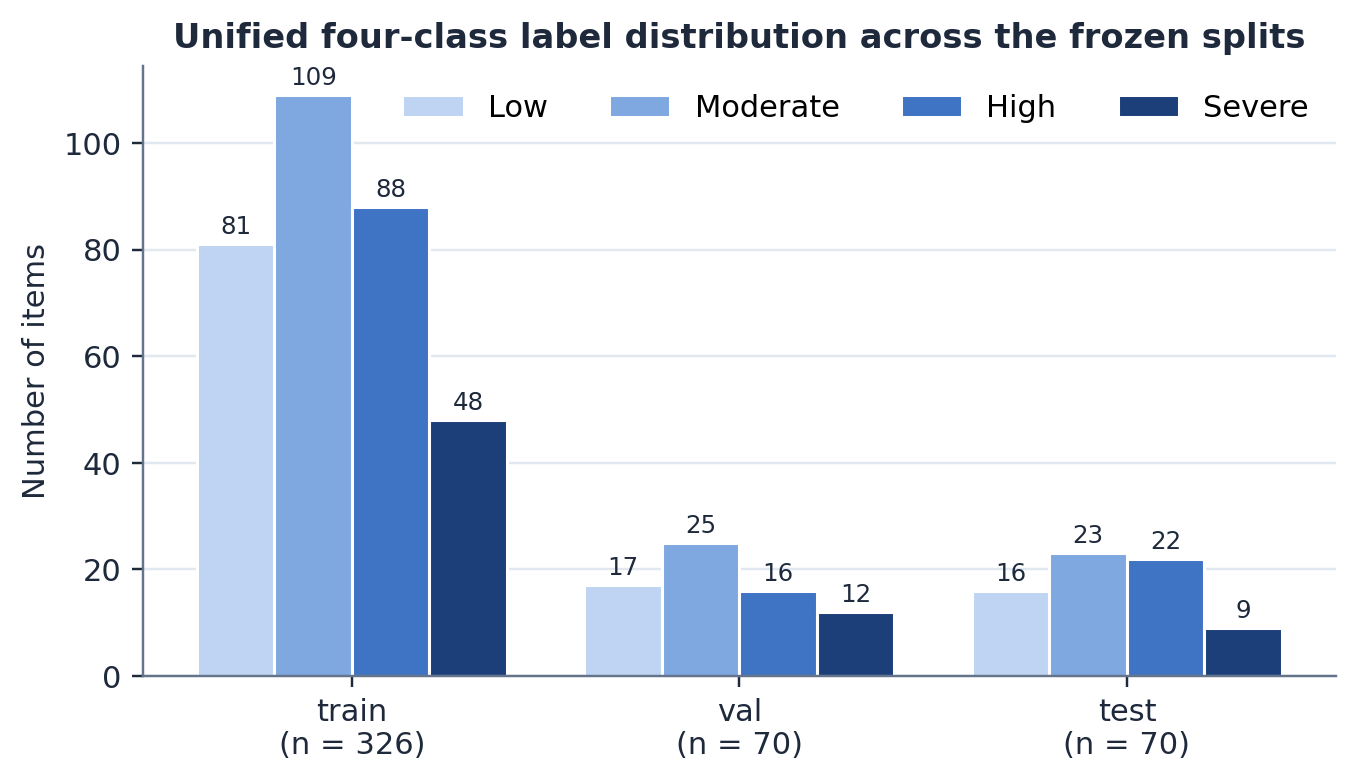
\includegraphics[width=0.85\linewidth]{fig_label_distribution.png}
	\caption{Label distribution across the frozen train, validation and test splits.}
	\label{fig:labels}
\end{figure}

\subsection{Protocol}
The systems, ablation configurations and metrics are those defined in Section~\ref{sec:eval-design}, with the hyperparameters of Table~\ref{tab:hyper}.

\section{Experiment Result}

\subsection{PhoBERT fine-tuning}
Training loss fell monotonically over four epochs (0.981, 0.668, 0.530, 0.489), while validation macro-F1 rose from 0.778 to 0.840 at epoch~2 and then plateaued (Figure~\ref{fig:training}); the epoch-2 checkpoint was kept. On its own three-class task the model reached \textbf{test accuracy 0.800 and macro-F1 0.801} (Table~\ref{tab:phobert3}). All 14 errors fall between adjacent classes (Figure~\ref{fig:confusion}b); none crosses from Low to High or back, which is the benign error pattern for an ordinal construct.

\begin{figure}[ht]
	\centering
	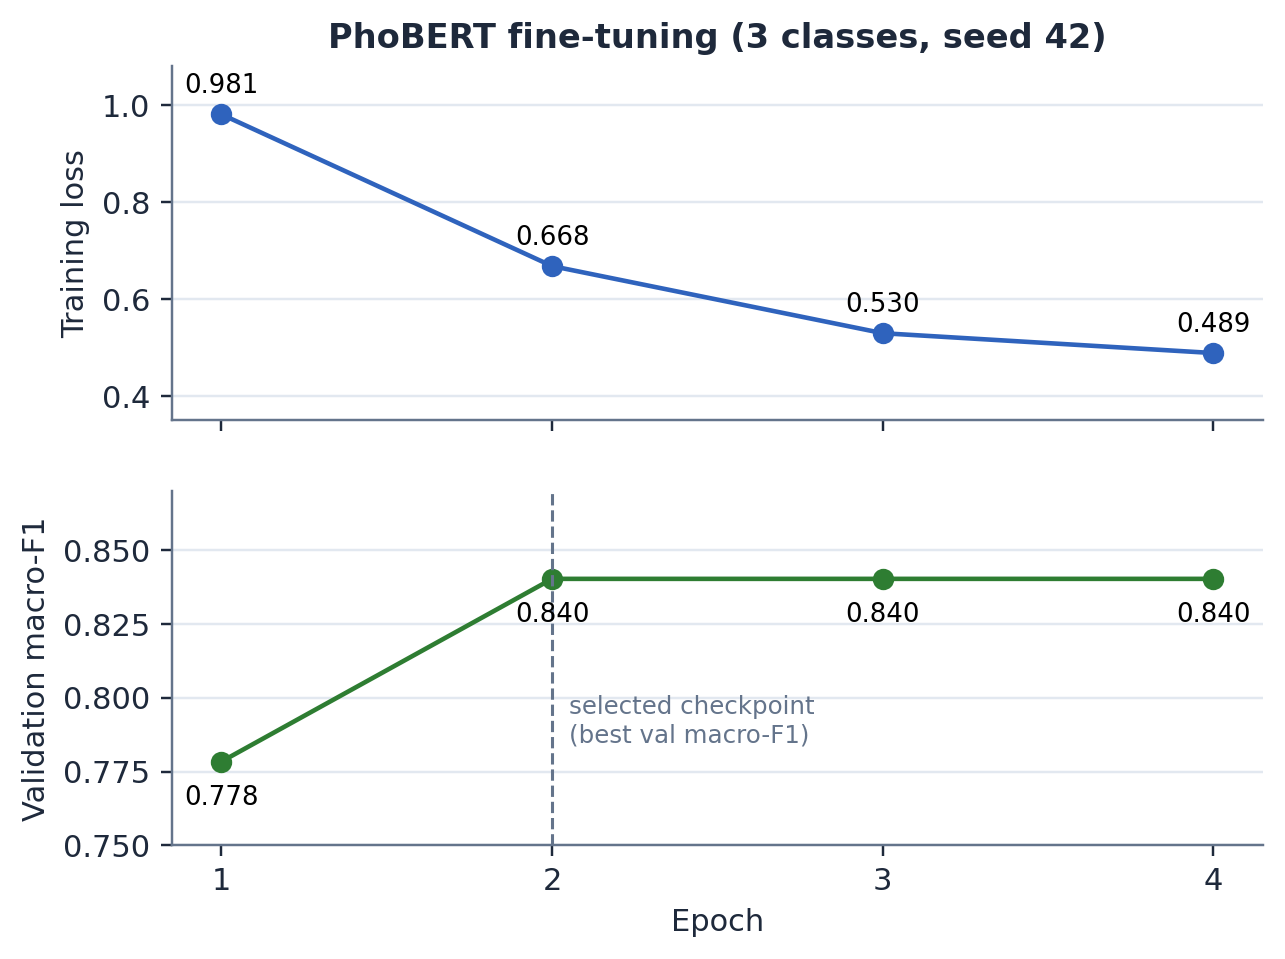
\includegraphics[width=0.72\linewidth]{fig_training_curves.png}
	\caption{PhoBERT training loss and validation macro-F1 per epoch.}
	\label{fig:training}
\end{figure}

\begin{table}[ht]
	\centering
	\caption{Fine-tuned PhoBERT on its three-class test split ($n=70$).}
	\label{tab:phobert3}
	\begin{tabular}{lrrrr}
		\toprule
		Class         & Precision      & Recall         & F1             & Support     \\ \midrule
		Low           & 0.818          & 0.947          & 0.878          & 19          \\
		Moderate      & 0.667          & 0.727          & 0.696          & 22          \\
		High          & 0.917          & 0.759          & 0.830          & 29          \\ \midrule
		Macro average & \textbf{0.801} & \textbf{0.811} & \textbf{0.801} & \textbf{70} \\ \bottomrule
	\end{tabular}
\end{table}

\subsection{Classification systems}
Table~\ref{tab:main} and Figure~\ref{fig:systems} compare all six systems on the unified four-class test split.

\begin{table}[ht]
	\centering
	\caption[Main results on the unified four-class test split]{Main results on the unified four-class test split ($n=70$, synthetic data, single seed). Best value per column in bold.}
	\label{tab:main}
	\resizebox{\textwidth}{!}{%
		\begin{tabular}{lrrrrrrr}
			\toprule
			System                     & Accuracy        & Macro-F1        & Cohen's $\kappa$ & F1 Low          & F1 Moderate     & F1 High         & F1 Severe       \\ \midrule
			Majority class             & 0.329           & 0.124           & 0.000            & 0.000           & 0.495           & 0.000           & 0.000           \\
			TF-IDF + LogReg            & \textbf{0.686}  & \textbf{0.682}  & \textbf{0.581}   & 0.821           & 0.651           & 0.588           & \textbf{0.667}  \\
			TF-IDF + SVM               & 0.657           & 0.652           & 0.542            & 0.821           & 0.622           & 0.500           & \textbf{0.667}  \\
			PhoBERT fine-tuned         & 0.657           & 0.533           & 0.516            & \textbf{0.842}  & \textbf{0.681}  & \textbf{0.609}  & 0.000$^\dagger$ \\
			LLM zero-shot              & 0.529           & 0.524           & 0.389            & \textbf{0.842}  & 0.375           & 0.316           & 0.563           \\
			Proposed pipeline          & 0.486           & 0.500           & 0.311            & 0.733           & 0.606           & 0.353           & 0.308           \\ \bottomrule
		\end{tabular}%
	}
	\par\smallskip
	{\raggedright\footnotesize $^\dagger$ PhoBERT has three output classes and cannot predict Severe.\par}
\end{table}

\begin{figure}[ht]
	\centering
	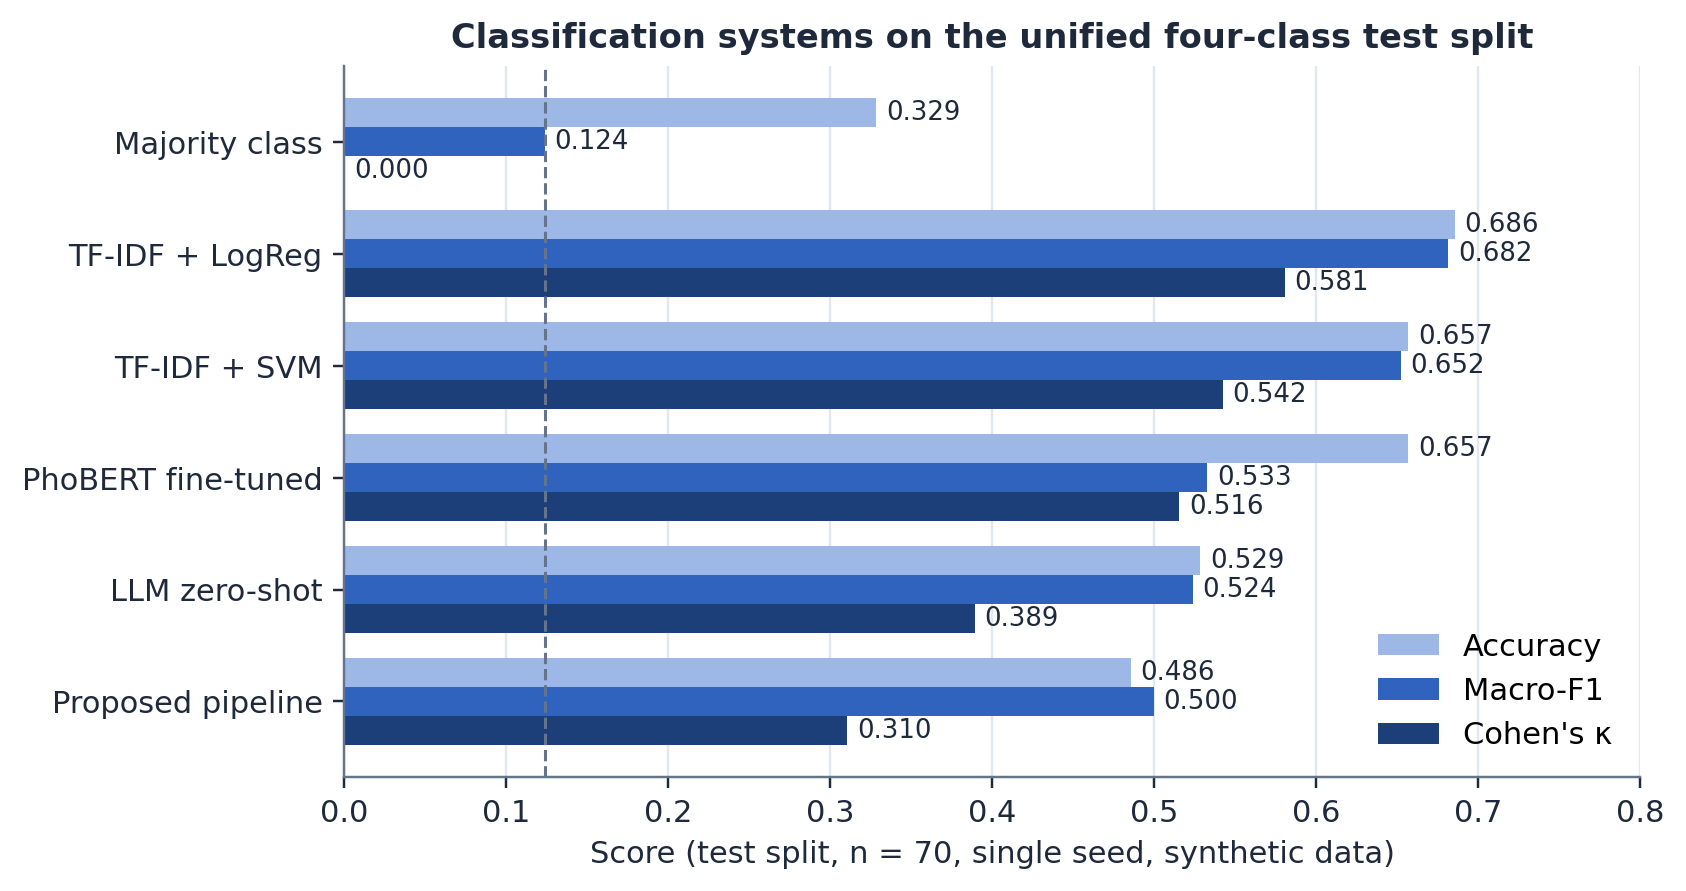
\includegraphics[width=0.95\linewidth]{fig_system_comparison.png}
	\caption{Accuracy, macro-F1 and Cohen's $\kappa$ per system. Dashed line: majority-class macro-F1.}
	\label{fig:systems}
\end{figure}

Four observations follow. \textbf{(1)~The classical TF-IDF baseline has the highest macro-F1 of any system}, including the proposed pipeline. \textbf{(2)~The proposed pipeline does not outperform zero-shot prompting} (0.500 against 0.524); this run is free of the two confounds that invalidated an earlier run (a retrieval query that differed from the deployed app on 53\,\% of items, and a quota cap that left 46\,\% of items unanswered). \textbf{(3)~PhoBERT's deficit is entirely in the Severe class}: on the three classes it can predict, its F1 equals or exceeds TF-IDF on every one (Figure~\ref{fig:perclass}). \textbf{(4)~Every system clears the majority-class floor}, so each learns something from its input. Figure~\ref{fig:confusion} shows that TF-IDF errors are also almost all adjacent: 21 of its 22 errors fall into a neighbouring class.

\begin{figure}[ht]
	\centering
	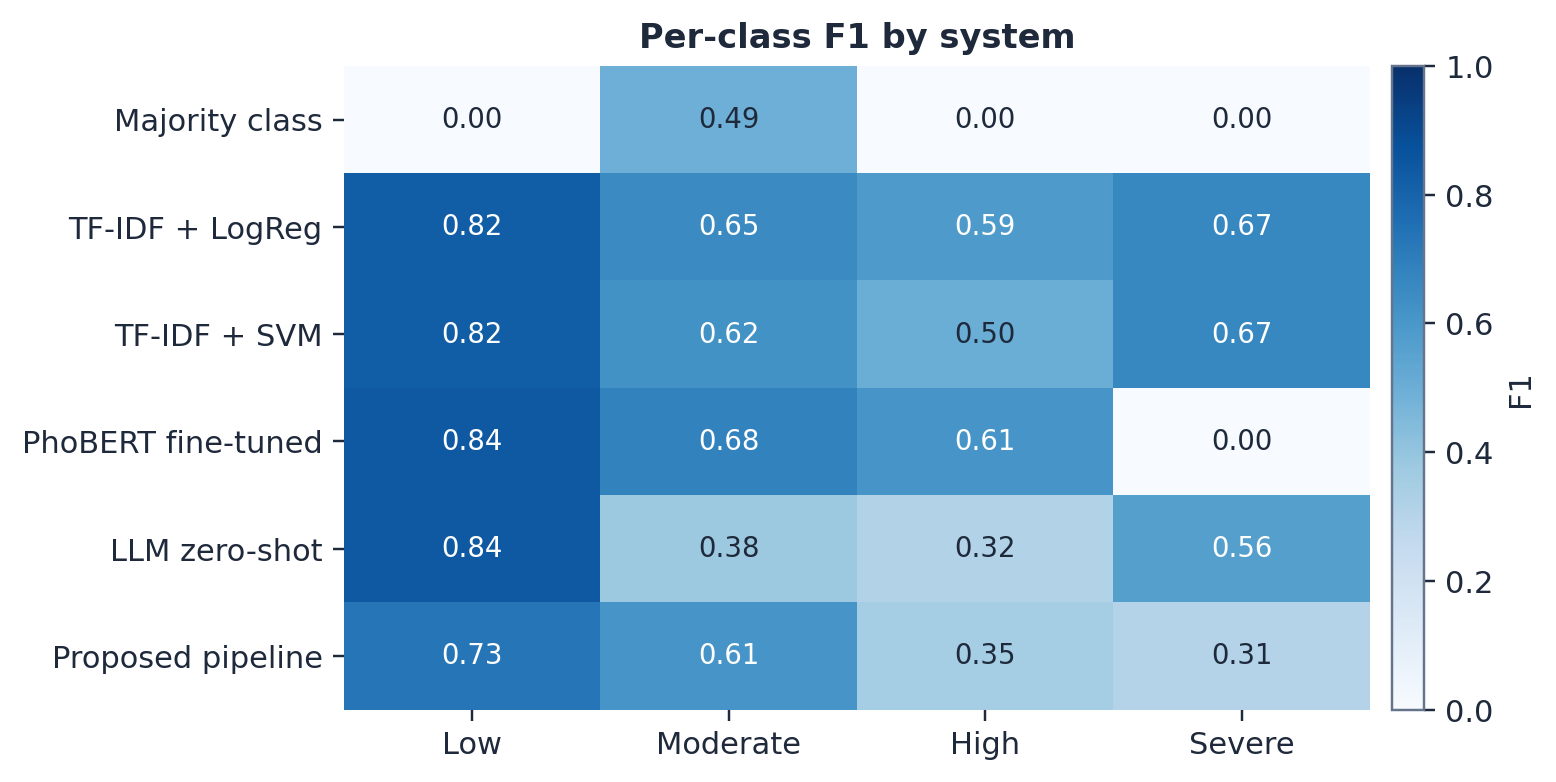
\includegraphics[width=0.78\linewidth]{fig_per_class_f1.png}
	\caption{Per-class F1 for every system.}
	\label{fig:perclass}
\end{figure}

\begin{figure}[ht]
	\centering
	\begin{minipage}{0.49\linewidth}
		\centering
		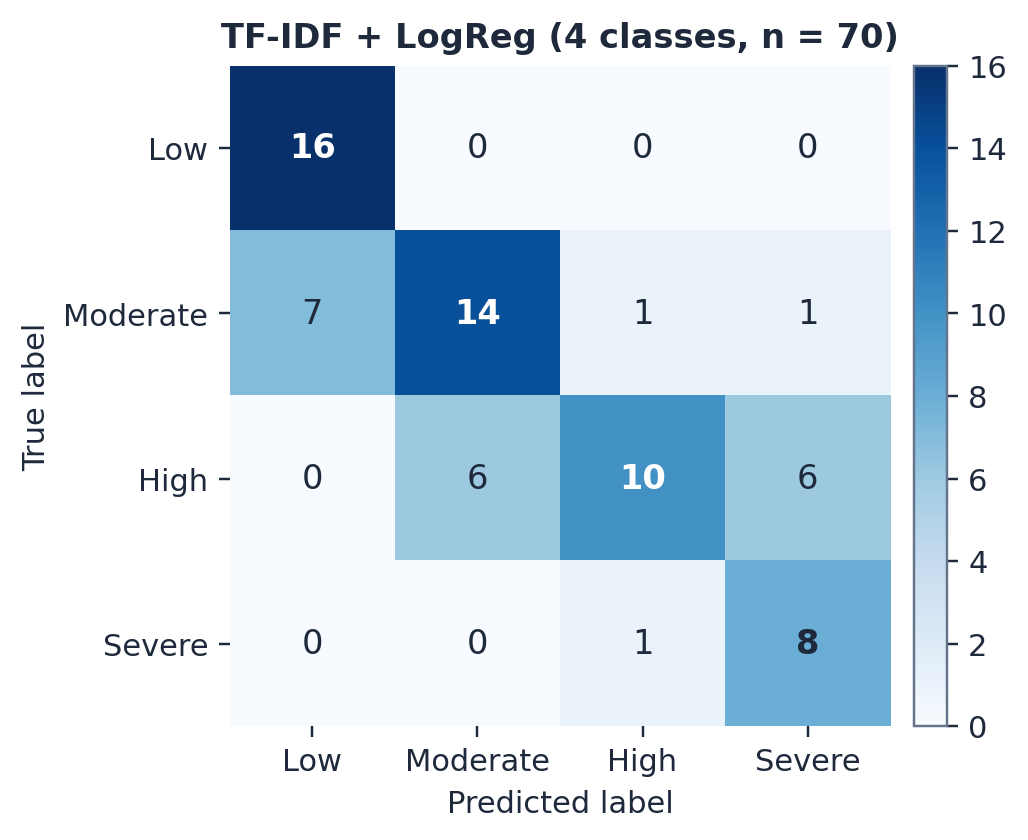
\includegraphics[width=\linewidth]{fig_confusion_tfidf_lr.png}\\
		\small (a) TF-IDF + LogReg, four classes
	\end{minipage}\hfill
	\begin{minipage}{0.49\linewidth}
		\centering
		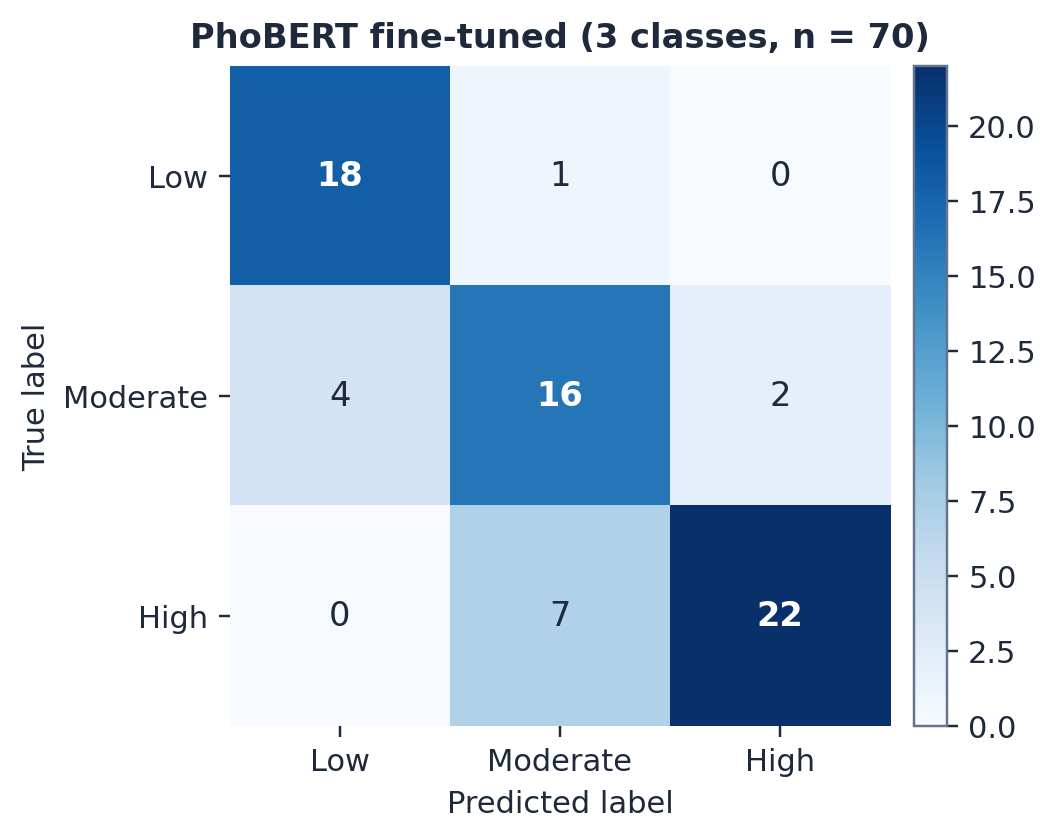
\includegraphics[width=\linewidth]{fig_confusion_phobert.png}\\
		\small (b) PhoBERT, three classes
	\end{minipage}
	\caption{Confusion matrices on the test split (rows: true label; columns: predicted label).}
	\label{fig:confusion}
\end{figure}

\subsection{Ablation}
\label{sec:res-ablation}
Three of the five configurations were run on a stratified 40-item subsample (Table~\ref{tab:ablation}, Figure~\ref{fig:ablation}).

\begin{table}[ht]
	\centering
	\caption[Ablation of proposed-pipeline components]{Ablation of proposed-pipeline components ($n=40$; noise floor $\pm0.148$). Quest.: questionnaire scores; Acc.: accuracy; $\Delta$: change in macro-F1 against \code{full}.}
	\label{tab:ablation}
	\begin{tabular}{lcccrrr}
		\toprule
		Configuration            & RAG    & Quest.        & Emotion & Acc.     & Macro-F1 & $\Delta$          \\ \midrule
		\code{full}              & \cmark & \cmark        & \cmark  & 0.525    & 0.534    & -               \\
		\code{no\_questionnaire} & \cmark & \xmark        & \cmark  & 0.325    & 0.123    & $\mathbf{-0.411}$ \\
		\code{no\_emotion}       & \cmark & \cmark        & \xmark  & 0.600    & 0.593    & $+0.059$          \\
		\code{no\_rag}           & \xmark & \cmark        & \cmark  & \multicolumn{3}{c}{not run} \\
		\code{text\_only}        & \xmark & \xmark        & \xmark  & \multicolumn{3}{c}{not run} \\ \bottomrule
	\end{tabular}
\end{table}

\begin{figure}[ht]
	\centering
	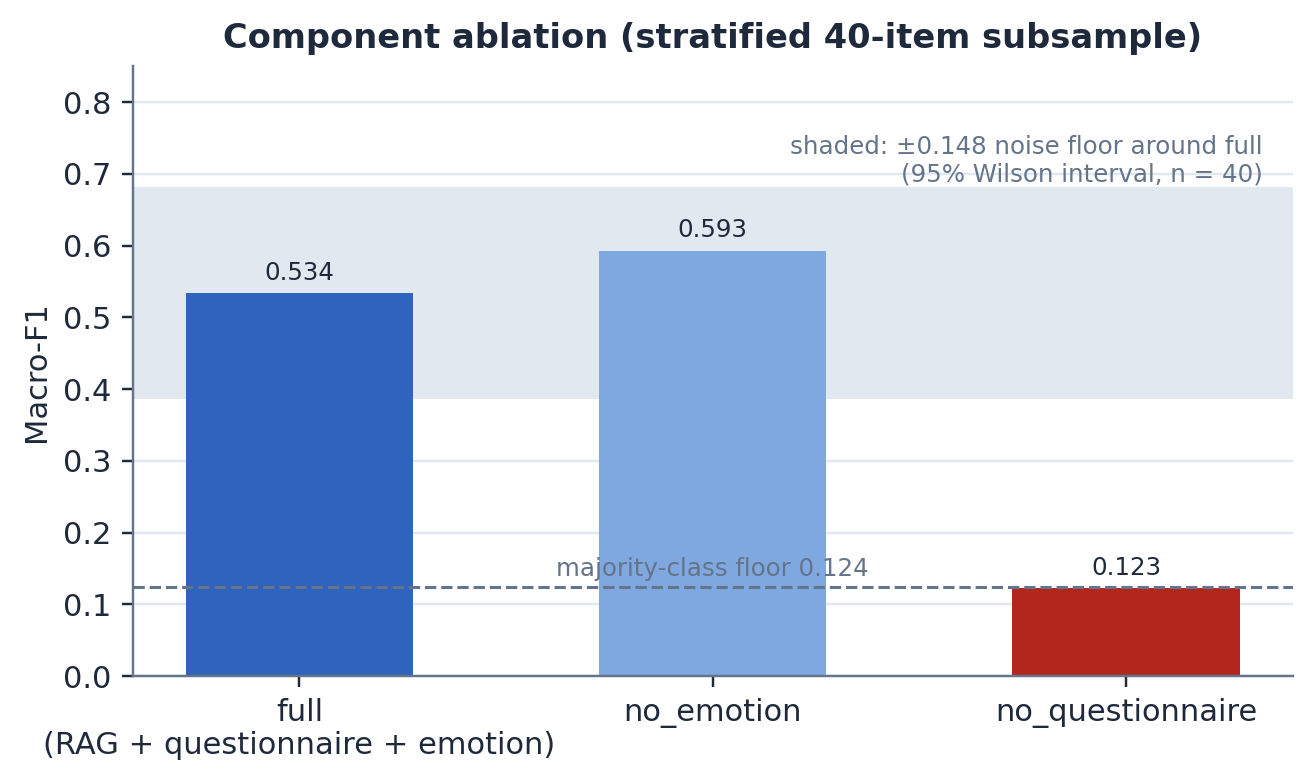
\includegraphics[width=0.8\linewidth]{fig_ablation.png}
	\caption{Macro-F1 per ablation configuration with the sampling noise floor and the majority-class floor.}
	\label{fig:ablation}
\end{figure}

\textbf{Removing the questionnaire scores is the one unambiguous result}: macro-F1 falls to 0.123, exactly the majority-class floor. Because those scores define the ground-truth label, this measures label leakage as much as feature value: substantially all of the pipeline's apparent agreement comes from being shown the quantities that define the answer. \textbf{Removing the text-analysis features changes nothing measurable}; the $+0.059$ is inside the noise floor, so no direction is claimed. The two retrieval-disabled configurations did not produce reportable results. Without retrieved material the model correctly obeyed the grounding rule and returned no suggestions, but the output schema requires at least one, so 29 of 40 \code{text\_only} replies (72\,\%) were rejected and the harness recorded the configuration as not run. This is a mismatch between the grounding rule and the schema, not a model failure.

\subsection{Retrieval quality}
\label{sec:res-rag}
Table~\ref{tab:retrieval} and Figure~\ref{fig:retrieval} report retrieval over the 57 labelled queries through the production \code{retrieve()} function. \textbf{MRR is 0.787}; at the production depth $k=4$, Recall lies between the $k=3$ and $k=5$ values of 0.838 and 0.903.

\begin{table}[ht]
	\centering
	\caption{Retrieval quality over 57 labelled queries (binary relevance).}
	\label{tab:retrieval}
	\begin{tabular}{rrrr}
		\toprule
		$k$ & Recall@$k$ & Precision@$k$ & nDCG@$k$ \\ \midrule
		1   & 0.658      & 0.684         & 0.684    \\
		3   & 0.838      & 0.298         & 0.776    \\
		5   & 0.903      & 0.200         & 0.807    \\
		8   & 0.965      & 0.136         & 0.829    \\ \bottomrule
	\end{tabular}
\end{table}

\begin{figure}[ht]
	\centering
	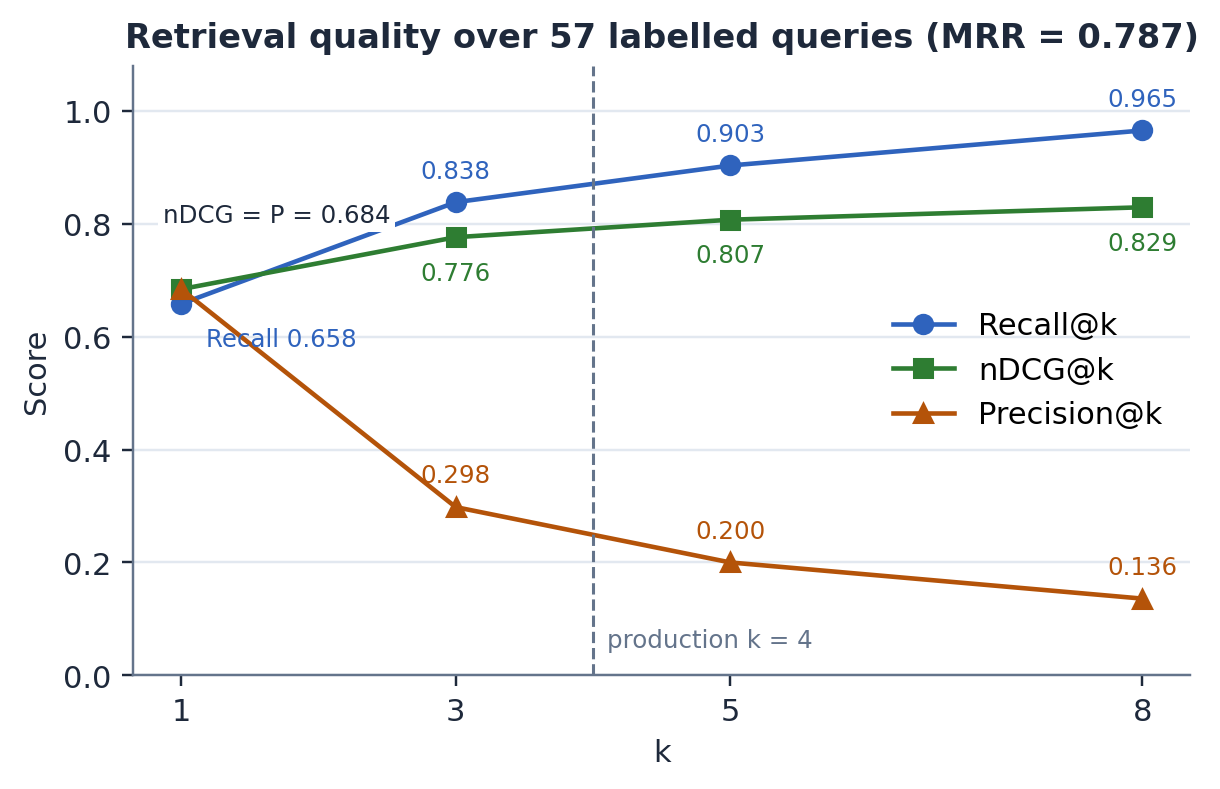
\includegraphics[width=0.75\linewidth]{fig_retrieval_at_k.png}
	\caption{Recall, precision and nDCG as a function of retrieval depth $k$.}
	\label{fig:retrieval}
\end{figure}

\textbf{The key finding concerns the query construction, and it changed the system.} The original \code{build\_rag\_query} discarded the student's sentence, retrieved on the matched lexicon keywords, and appended a label string. A paired comparison - the same queries and relevance labels under six candidate constructions - was run. On the 16 queries the construction actually alters (Table~\ref{tab:query}, Figure~\ref{fig:query}), the sentence alone beat the keywords alone (MRR 0.778 against 0.509), and appending the label hurt every variant, costing the best one 0.15 MRR. The construction was rewritten to keep the sentence and append the keywords, which outperforms even the sentence alone. Vietnamese and English queries score similarly (MRR 0.800 and 0.786), though only five queries are Vietnamese. Six queries retrieved nothing relevant in the top four; one is safety-relevant (\textit{``hopeless worthless lost motivation''} missed the help-seeking and counselling sections).

\begin{table}[ht]
	\centering
	\caption[Paired comparison of query constructions]{Paired comparison of query constructions on the 16 affected queries. Old: matched keywords plus a label string; Sentence: the student's sentence only; Current: sentence plus matched keywords.}
	\label{tab:query}
	\begin{tabular}{lrrrr}
		\toprule
		Metric   & Old                   & Sentence      & \textbf{Current}                      & $\Delta$ vs.\ old \\ \midrule
		MRR      & 0.509                 & 0.778         & \textbf{0.839}                        & $+0.329$          \\
		Recall@1 & 0.344                 & 0.656         & \textbf{0.719}                        & $+0.375$          \\
		Recall@5 & 0.688                 & 0.938         & \textbf{1.000}                        & $+0.312$          \\
		nDCG@5   & 0.540                 & 0.809         & \textbf{0.879}                        & $+0.338$          \\ \bottomrule
	\end{tabular}
\end{table}

\begin{figure}[ht]
	\centering
	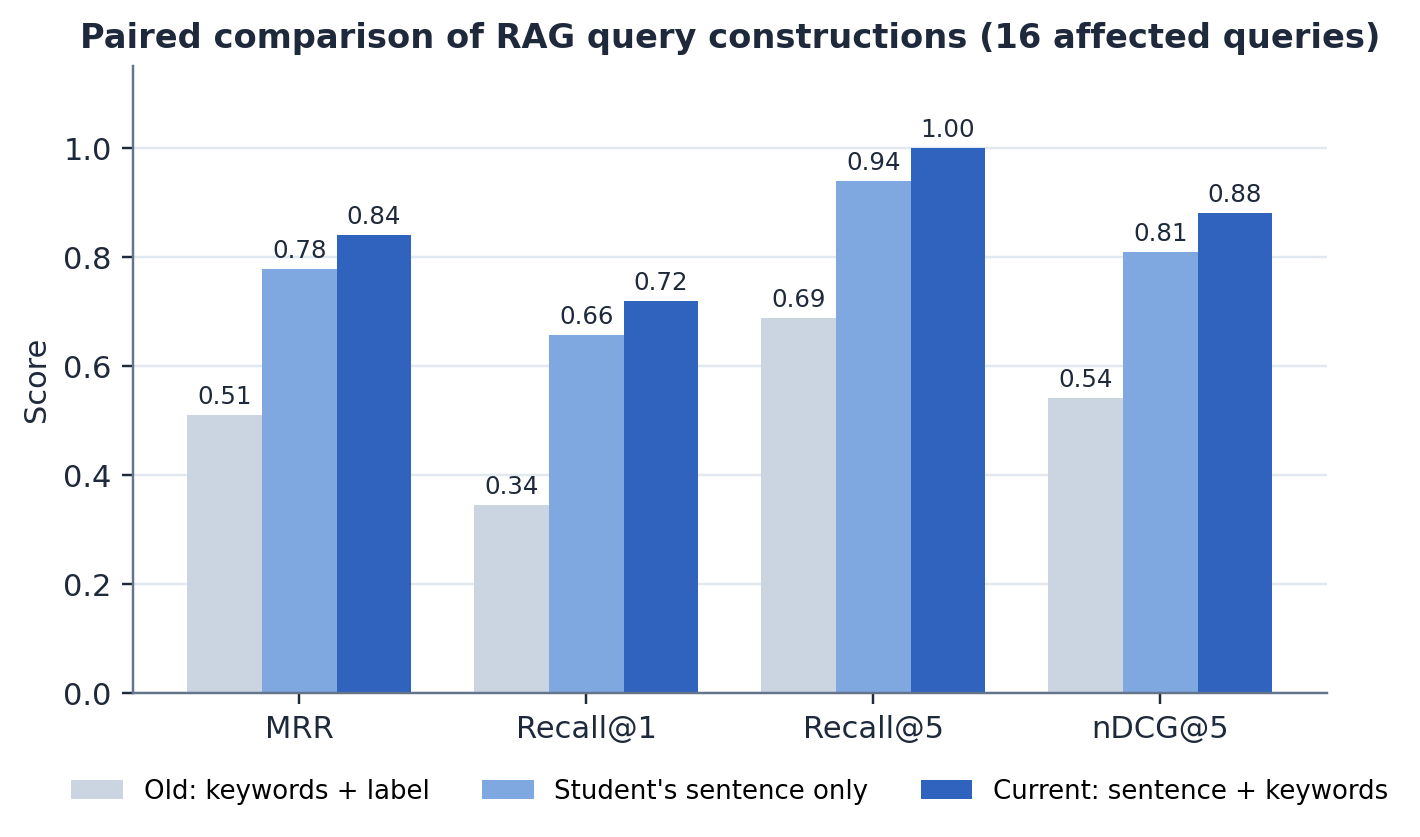
\includegraphics[width=0.85\linewidth]{fig_query_construction.png}
	\caption{Effect of query construction on retrieval (paired design).}
	\label{fig:query}
\end{figure}

\subsection{Crisis detection}
Table~\ref{tab:crisis} compares the original phrase-list rule with the construct-based rule on all three sets, and Figure~\ref{fig:crisis} visualises it. \textbf{Only the held-out row is evidence}: the two development sets were used for debugging, so their post-rebuild scores are fitted by construction and are shown for completeness only. On the held-out set, precision rose from 0.600 to \textbf{1.000} and recall from 0.200 to \textbf{0.867}, with indirect ideation detected in 11 of 14 items instead of none. After fixing regressions found on the development sets, the held-out set was re-measured and produced identical numbers.

\begin{table}[ht]
	\centering
	\caption{Crisis-detection rule before and after the rebuild.}
	\label{tab:crisis}
	\resizebox{\textwidth}{!}{%
		\begin{tabular}{llrrrrr}
			\toprule
			Set                                  & Rule            & Precision      & Recall         & F1             & Explicit       & Indirect       \\ \midrule
			\textbf{Held-out} (60, bilingual)    & phrase list     & 0.600          & 0.200          & 0.300          & 6/12           & 0/14           \\
			                                     & \textbf{constructs} & \textbf{1.000} & \textbf{0.867} & \textbf{0.929} & \textbf{12/12} & \textbf{11/14} \\ \midrule
			VI development (50)                  & phrase list     & 0.800          & 0.500          & 0.615          & 10/10          & 1/9            \\
			                                     & constructs      & 1.000          & 1.000          & 1.000          & 10/10          & 9/9            \\ \midrule
			EN development (50)                  & phrase list     & 1.000          & 0.417          & 0.588          & 10/10          & 0/10           \\
			                                     & constructs      & 1.000          & 0.833          & 0.909          & 10/10          & 7/10           \\ \bottomrule
		\end{tabular}%
	}
\end{table}

\begin{figure}[ht]
	\centering
	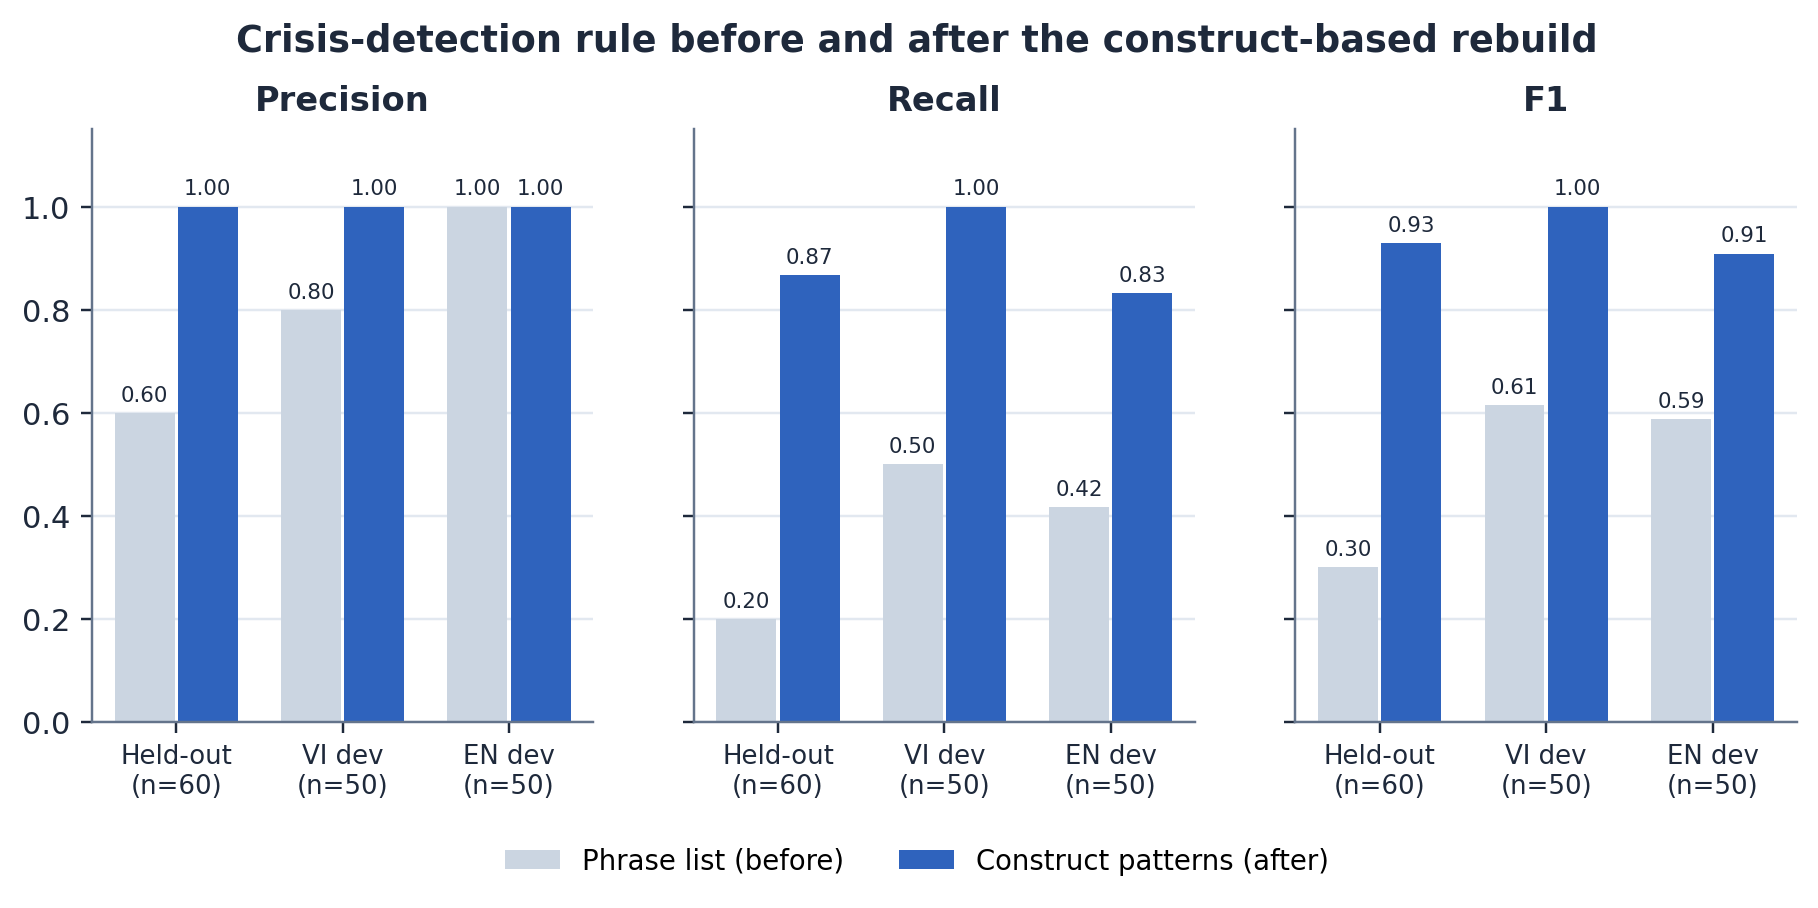
\includegraphics[width=0.95\linewidth]{fig_crisis_before_after.png}
	\caption{Precision, recall and F1 of the crisis rule before and after the rebuild.}
	\label{fig:crisis}
\end{figure}

On the held-out set the rule produced TP~26, FP~0, FN~4 and TN~30 (Figure~\ref{fig:crisis-cat}). It raised no false positive on any of the 51 deliberately lethal-sounding hard negatives across the three sets. The four held-out misses - a railing on the ninth floor (in both languages), counting pills, and hoping something happens - are listed verbatim in Appendix~\ref{app:crisis}.

\begin{figure}[ht]
	\centering
	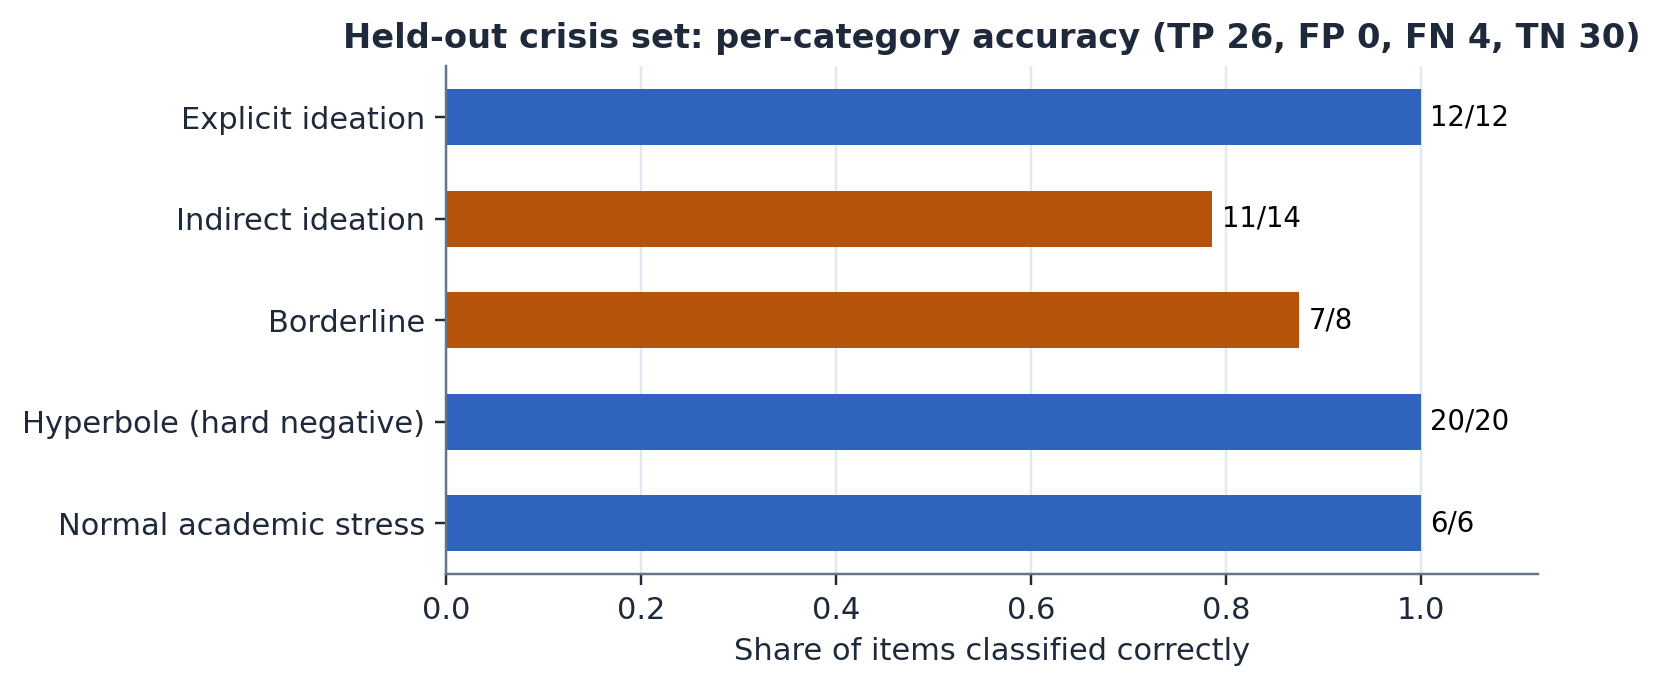
\includegraphics[width=0.8\linewidth]{fig_crisis_categories.png}
	\caption{Held-out crisis set: accuracy per category.}
	\label{fig:crisis-cat}
\end{figure}

\subsection{Latency}
Table~\ref{tab:latency} and Figure~\ref{fig:latency} report 30 timed runs of each deterministic stage. The whole deterministic path costs \textbf{under 90\,ms at p50}, and the crisis gate that precedes every side effect costs 0.05\,ms. Cold start is paid once per process: 10.8\,s for PhoBERT and 10.8\,s for the embedder. End-to-end latency including generation, tokens per session and cost were not measured, because each sample is a billable request and the day's quota was used by the comparison run; on the Groq free tier the monetary cost is zero and the binding limit is the daily token cap.

\begin{table}[ht]
	\centering
	\caption{Latency per stage (ms, CPU, $n=30$).}
	\label{tab:latency}
	\begin{tabular}{lrr}
		\toprule
		Stage                                  & p50               & p95                \\ \midrule
		DASS-21 + PSS-10 scoring               & 0.03              & 0.05               \\
		Crisis rule                            & 0.05              & 0.07               \\
		Lexicon keyword match                  & 0.07              & 0.12               \\
		RAG retrieval ($k=4$)                  & 28.01             & 83.43              \\
		PhoBERT inference                      & 59.31             & 93.32              \\ \midrule
		\textbf{Deterministic path, total}     & $\mathbf{\approx 88}$ & $\mathbf{\approx 177}$ \\
		Cold start: PhoBERT / embedder (once)  & 10,820 / 10,829   & -                \\
		End-to-end with generation             & \multicolumn{2}{c}{not measured}       \\ \bottomrule
	\end{tabular}
\end{table}

\begin{figure}[ht]
	\centering
	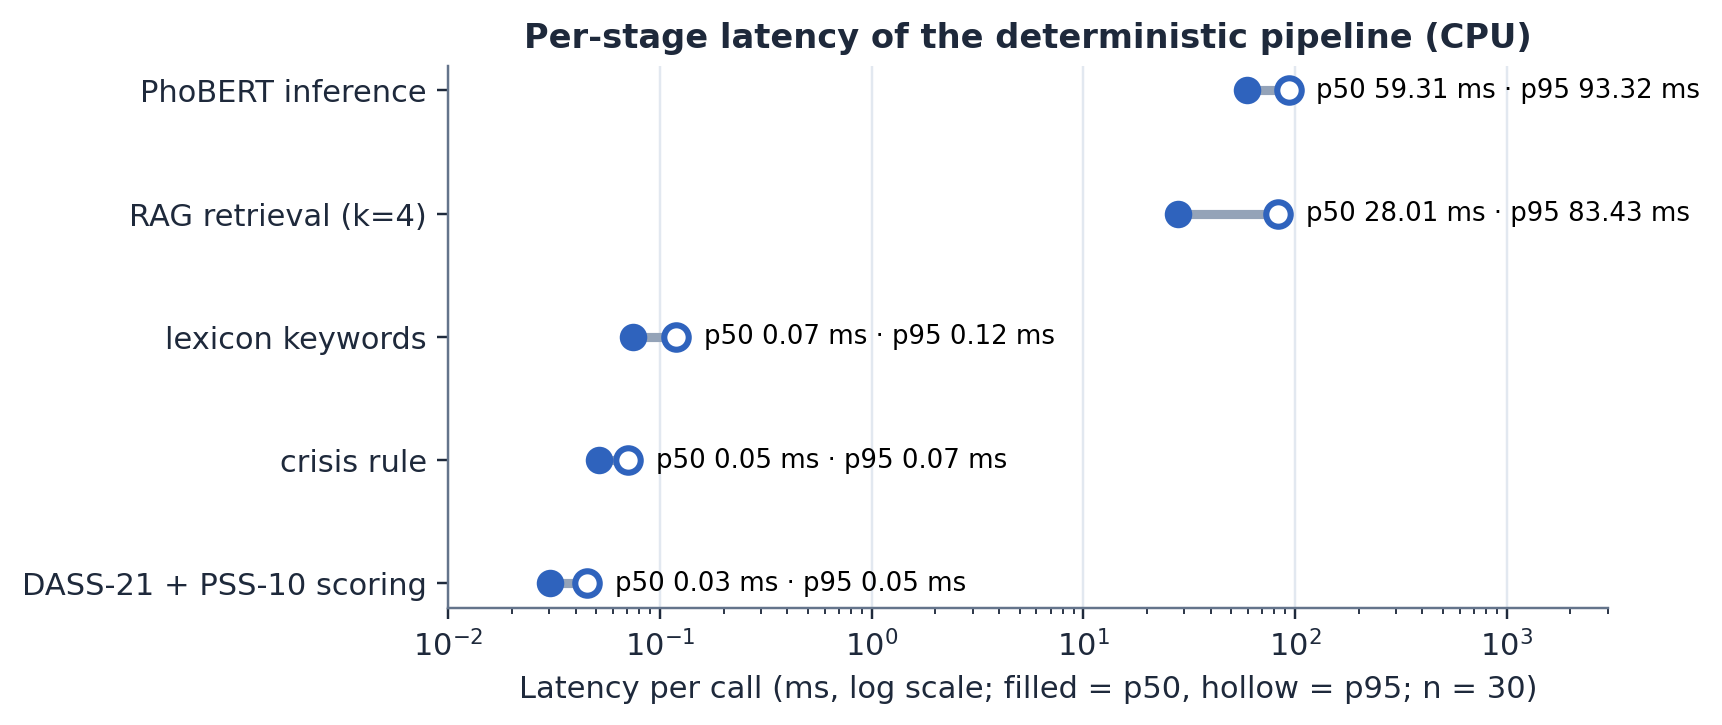
\includegraphics[width=0.85\linewidth]{fig_latency.png}
	\caption{Per-stage latency, p50 to p95, on a logarithmic axis.}
	\label{fig:latency}
\end{figure}

\subsection{Data leakage and label ceiling}
\label{sec:res-leakage}
The exact-duplicate check passes: 0 of 70 test texts appear in the training split. The near-duplicate measurement tells a different story (Table~\ref{tab:leakage}, Figure~\ref{fig:leakage}). The median similarity of a test text to its nearest training text is \textbf{0.799}, and \textbf{34 of 70} test items exceed 0.80. Two further similarity measures agree, so the conclusion is not an artefact of one metric.

\begin{table}[ht]
	\centering
	\caption{Nearest-neighbour similarity of each test item to the training split.}
	\label{tab:leakage}
	\begin{tabular}{lrrrrr}
		\toprule
		Measure               & Median & p90   & Max   & $>0.80$ & $>0.90$ \\ \midrule
		\code{difflib} ratio  & 0.799  & 0.893 & 0.907 & 34/70   & 4/70    \\
		Word TF-IDF cosine    & 0.797  & 0.892 & 0.946 & 34/70   & 5/70    \\
		Char TF-IDF cosine    & 0.806  & 0.901 & 0.931 & 37/70   & 8/70    \\ \bottomrule
	\end{tabular}
\end{table}

\begin{figure}[ht]
	\centering
	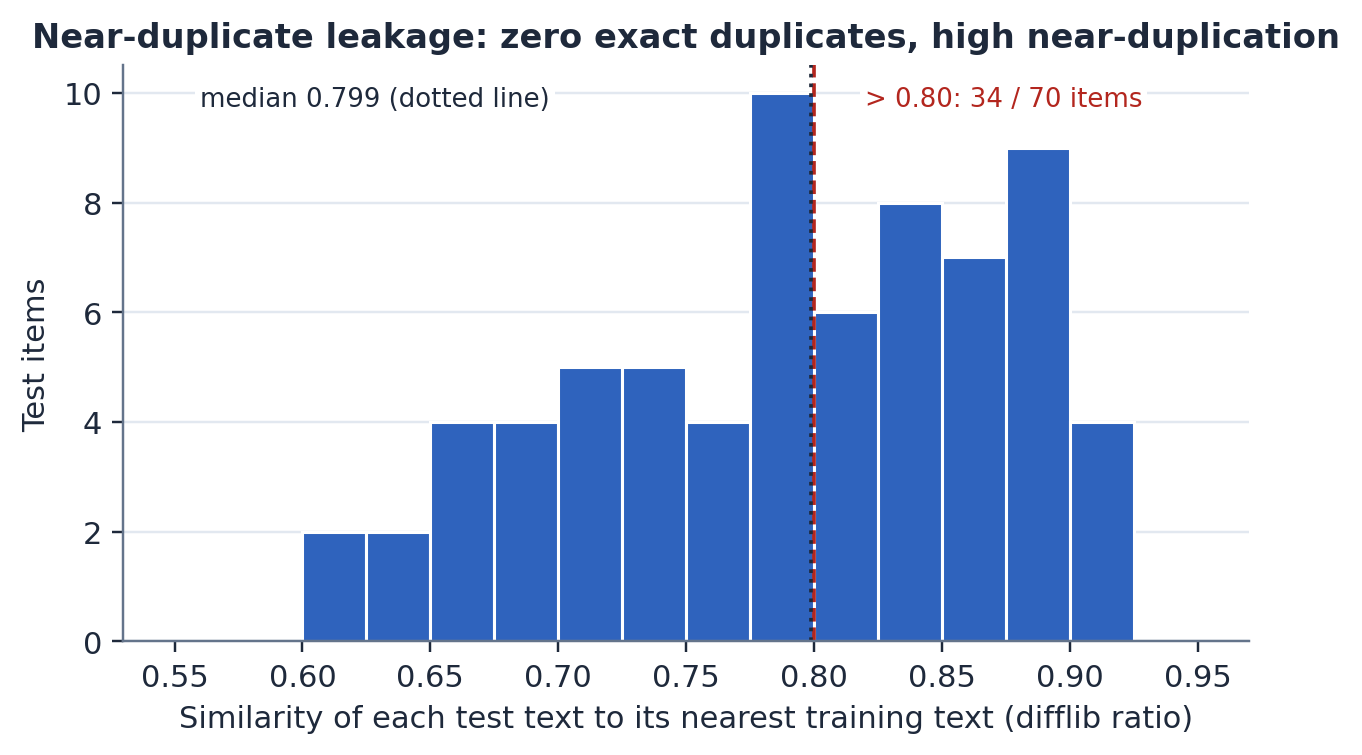
\includegraphics[width=0.8\linewidth]{fig_leakage.png}
	\caption{Distribution of nearest-neighbour similarity between test and training texts.}
	\label{fig:leakage}
\end{figure}

A second property bounds what any text-only classifier can achieve. The generator chooses a text's stress band by thresholding $\theta$, while the label comes independently from noisy questionnaire answers conditioned on $\theta$. The two disagree near the boundaries (Table~\ref{tab:band}): only \textbf{78.6\,\%} of test items (55 of 70) carry text from a band consistent with their label, so a classifier that perfectly recovered the text band would still score about 0.79 accuracy.

\begin{table}[ht]
	\centering
	\caption{Generated text band against questionnaire-derived label (all 466 items).}
	\label{tab:band}
	\begin{tabular}{lrrrr}
		\toprule
		Text band $\downarrow$ / Label $\rightarrow$ & Low & Moderate & High & Severe \\ \midrule
		low                                          & 109 & 35       & 2    & 0      \\
		moderate                                     & 5   & 116      & 39   & 5      \\
		high                                         & 0   & 6        & 85   & 64     \\ \bottomrule
	\end{tabular}
\end{table}

\subsection{Summary of unmeasured quantities}
Table~\ref{tab:notrun} lists what this pre-thesis did not measure, so that no gap is mistaken for a result.

\begin{table}[ht]
	\centering
	\caption{Quantities specified in the evaluation design but not yet measured.}
	\label{tab:notrun}
	\begin{tabularx}{\textwidth}{lL}
		\toprule
		Quantity                                      & Reason / dependency \\ \midrule
		RAG faithfulness (LLM-as-judge + human subset) & Needs generated answers at scale and provider quota \\
		\code{no\_rag} and \code{text\_only} ablations & Blocked by the schema requiring at least one suggestion \\
		End-to-end latency, tokens and cost per session & Each sample is a billable request \\
		Multi-seed variance, bootstrap CIs, McNemar's test & Not yet run \\
		Few-shot LLM and XLM-R baselines              & Not implemented \\
		LLM--questionnaire disagreement rate          & Needs stored predictions from real sessions \\
		Human evaluation (Krippendorff's $\alpha$) and SUS & Instruments implemented; no raters or participants yet \\
		Any result on real student text               & No participant data collected \\ \bottomrule
	\end{tabularx}
\end{table}


\chapter{DISCUSSION}\label{ch:discussion}
This chapter interprets the results of Chapter~\ref{ch:result}, states the strengths and limitations of the work, positions it against related work, and sets out future work.

\section{Analysis}

\subsection{Why the classical baseline wins}
The headline result is uncomfortable and should be stated plainly: \textbf{a TF-IDF linear model outperforms the fine-tuned Vietnamese transformer} on the four-class task (macro-F1 0.682 against 0.533). Three factors explain this, and separating them matters.

\textbf{A structural class deficit.} PhoBERT has three output classes and the evaluation space has four. Its F1 on Severe is zero by construction, which alone can lower a four-class macro average by up to 0.25. On the three classes it can predict, it matches or beats TF-IDF on every one (0.842 vs.\ 0.821 on Low, 0.681 vs.\ 0.651 on Moderate, 0.609 vs.\ 0.588 on High). Retraining with four classes is the correct remedy.

\textbf{An intrinsic label ceiling.} Because text band and label are separate noisy functions of the latent variable (Table~\ref{tab:band}), a perfect text-band classifier would score only about 0.79 accuracy. TF-IDF's 0.686 therefore recovers roughly 87\,\% of the recoverable signal, and most of the apparent headroom is illusory. This also explains PhoBERT's higher score on its own three-class task, whose label is better aligned with the text band.

\textbf{The register of the data.} Template-generated text is a distribution over recurring phrases, for which word bigrams are close to ideal. A transformer's strengths - paraphrase, composition, context - have nothing to work on. This is the factor expected to reverse on real student writing, and the near-duplicate measurement (34 of 70 test items above 0.80 similarity) confirms that the task being measured is largely template recognition.

\subsection{Error analysis}
Of the 22 TF-IDF errors, 21 are between adjacent classes. The dominant confusions are Moderate predicted as Low (7), High predicted as Moderate (6) and High predicted as Severe (6). Two representative errors:

\begin{enumerate}
	\item \textit{``\vi{Tâm trạng mình dạo này khá tốt. Bài vở không quá nhiều nên mình có thời gian nghỉ ngơi.}''} (``My mood has been quite good lately. There is not too much coursework so I have time to rest.'') - true \textbf{Moderate}, predicted \textbf{Low}. The prediction is arguably the correct reading of the text; the error comes from the label-noise mechanism above.
	\item \textit{``\vi{Mấy tuần nay mình thấy hơi quá tải. Chủ yếu là do bài tập và deadline dồn dập.}''} (``These past weeks I have felt a bit overloaded, mainly because of piled-up assignments and deadlines.'') - true \textbf{High}, predicted \textbf{Moderate}. Hedging language (\vi{hơi quá tải}, ``a bit overloaded'') accompanies high-stress content - precisely what a stronger text model should resolve.
\end{enumerate}

\subsection{The proposed pipeline and circularity}
The full pipeline scores below zero-shot prompting, and the ablation shows why its score should not be read as text understanding: without the questionnaire scores it falls to the majority-class floor. The LLM is therefore not adding classification value on this dataset. This is consistent with Strategy~3 (Section~4.2.3): the design already restricts the LLM to explanation and suggestions, and takes the headline from the validated instrument. The results support that decision rather than undermining it.

\subsection{Safety and retrieval}
The crisis rule shows that a pattern-based rule, organised by clinical construct rather than by fixed phrases, can move from detecting almost no indirect ideation to detecting most of it without losing precision. Its remaining misses (a balcony railing, counting pills) express risk through \textit{situations} rather than statements, which a pattern rule cannot generalise to; this is the natural boundary of the approach. The retrieval experiment is the clearest case in the project of a measurement changing the system: a plausible, never-questioned query construction was costing about a third of retrieval effectiveness wherever it fired.

\section{Strengths}
\begin{itemize}
	\item \textbf{A complete, working system.} Consent, two validated instruments, bilingual text analysis, grounded advice, history and deletion run end to end, with 341 passing tests and 94\,\% coverage of application code.
	\item \textbf{Safety by architecture, not by prompt.} The crisis gate is deterministic, costs 0.05\,ms, and runs before any storage or external call; crisis disclosures are never persisted.
	\item \textbf{The validated instrument owns the headline}, and the LLM cannot silently override it.
	\item \textbf{Grounding checked in code.} Citations are verified against what was retrieved, and generation is refused when nothing is retrieved.
	\item \textbf{Methodological honesty.} The crisis held-out set was frozen before the rule was written; gaps are recorded as ``not run'' instead of estimated; unflattering results are reported as they are.
	\item \textbf{Graceful degradation.} Every unreliable component can fail without the student losing their questionnaire result.
	\item \textbf{Low operating cost.} The deterministic path runs on CPU in under 90\,ms, and the configured LLM provider's free tier costs nothing per session.
\end{itemize}

\section{Limitations}
\label{sec:limitations}

\subsection{Data}
\textbf{The dataset is the binding limitation.} Training \textit{and} evaluation text are synthetic, generated from 41 templates, and nearly half of the test items are near-copies of training items even though exact-duplicate leakage is zero. Every classification figure therefore measures template recognition and must not be read as evidence of stress-detection ability. No human participant has contributed data.

\subsection{Evaluation}
\begin{itemize}
	\item \textbf{Faithfulness is unmeasured.} Citations are verified, but whether a cited passage truly supports the sentence citing it has not been measured.
	\item \textbf{Single-author test sets.} The crisis held-out set and the retrieval query labels were written by the same person who built the system; there is no inter-annotator agreement.
	\item \textbf{No statistical treatment.} All results are single-seed, without confidence intervals or significance tests; the ablation uses only 40 items.
	\item \textbf{Two ablations did not run} because of the schema--grounding mismatch described in Section~\ref{sec:res-ablation}.
	\item \textbf{The English path of the classifier is unevaluated.} PhoBERT runs only on Vietnamese input, so English submissions use the lexicon path, which no classification experiment covers.
\end{itemize}

\subsection{Construct validity}
The four-level composite label (Equation~\eqref{eq:label}) is an invention of this project with no psychometric validation. The PSS-10 bands are a convention, not published clinical cut-offs. The knowledge base was written for this project rather than sourced from reviewed material, and no clinician has reviewed any output.

\subsection{Privacy and deployment}
Three gaps remain between the implementation and the consent instrument. The history endpoint is \textbf{unauthenticated}: protection rests on the unguessability of a random UUID, not on access control. The 12-month retention period is stated but \textbf{not enforced automatically}; deletion is participant-initiated only. Demographics (age, gender, year, major, university) are retained, so within a small programme the data is \textit{pseudonymous} rather than anonymous. The generative component is a third-party service whose behaviour may change without notice. \textbf{The system should not be deployed to real students} until the crisis rule is validated by an independent annotator, access control and automatic retention are in place, and institutional ethics review is complete, with a named human counsellor as the escalation route.

\section{Comparison}
Table~\ref{tab:compare} positions this work against published work. The figures are \textbf{not comparable}, and no claim of superiority or parity is made: the languages, label spaces, text registers, annotation processes and data provenance all differ, and this work's data is synthetic. The table is a positioning device, not a leaderboard.

\begin{table}[ht]
	\centering
	\caption{Positioning against published related work.}
	\label{tab:compare}
	\resizebox{\textwidth}{!}{%
		\begin{tabular}{lllll}
			\toprule
			Work                                  & Language   & Data                            & Task                          & Relation to this work \\ \midrule
			Turcan \& McKeown~\cite{turcan2019}   & English    & Reddit, human-annotated         & Binary stress                 & Closest task; different language, register, labels \\
			Coppersmith et al.~\cite{coppersmith2015} & English & Twitter, human-annotated        & Depression / PTSD             & Different construct and register \\
			Losada \& Crestani~\cite{losada2016}  & English    & Reddit, sequential              & Early risk detection          & No longitudinal data here \\
			Nguyen \& Nguyen~\cite{nguyen2020phobert} & Vietnamese & General Vietnamese benchmarks & POS, NER, NLI                 & Same encoder, different task \\
			Lewis et al.~\cite{lewis2020rag}      & English    & Wikipedia                       & Open-domain QA                & Same architecture, advisory use here \\ \midrule
			\textbf{This work}                    & \textbf{Vietnamese / English} & \textbf{Synthetic, 41 templates} & \textbf{4-level academic stress} & \textbf{Macro-F1 0.682 (TF-IDF), 0.533 (PhoBERT)} \\ \bottomrule
		\end{tabular}%
	}
\end{table}

What distinguishes this work is not a metric but a combination: validated psychometric scoring, Vietnamese text analysis, grounded generation with verified citations, and a measured bilingual crisis gate in one system (Table~\ref{tab:gap}).

\section{Future Work}
Items are ordered by expected evidential value relative to cost; the first two are planned for the thesis phase.

\begin{enumerate}
	\item \textbf{Run the real-data study.} The consent form, participant instructions, anonymised export, quality screening and an identical \code{--dataset real} evaluation path already exist. Recruiting 150--300 consenting students and re-running every evaluation would turn the classification results from a pipeline demonstration into evidence.
	\item \textbf{Validate the crisis rule independently.} Have an independent annotator write a new held-out set, measure once, and consider a small supervised classifier as a second, recall-oriented layer behind the pattern rule.
	\item \textbf{Measure faithfulness.} Add an LLM-as-judge rubric over at least 50 generated answers, with a 20-item human-labelled subset to measure judge--human agreement.
	\item \textbf{Fix the schema--grounding mismatch} by allowing an empty suggestion list with a stated reason, then run the \code{no\_rag} and \code{text\_only} ablations.
	\item \textbf{Retrain PhoBERT with four classes}, add XLM-R and few-shot LLM baselines, and run the word-segmentation ablation with VnCoreNLP applied at both training and inference.
	\item \textbf{Add statistical treatment}: three seeds with mean and standard deviation, bootstrap 95\,\% confidence intervals for macro-F1, and McNemar's test against the strongest baseline.
	\item \textbf{Tune retrieval}: a similarity threshold or a sweep of $k$ against faithfulness, and a better query for questionnaire-only submissions.
	\item \textbf{Close the privacy gaps}: authentication and encryption at rest for history, automatic 12-month expiry, and coarser demographics.
	\item \textbf{Human evaluation}: rate explanations for accuracy, helpfulness and respectfulness with three raters (Krippendorff's $\alpha$), and administer the SUS.
	\item \textbf{Clinician-in-the-loop review} of generated assessments and crisis decisions, and institutional ethics approval before any live use.
\end{enumerate}

Longer-term directions include multi-task prediction of the DASS-21 subscales instead of one composite, fully on-device inference to remove third-party transmission, and longitudinal tracking to detect change over a semester rather than a single point in time.


\chapter{CONCLUSION}\label{ch:conclusion}
This pre-thesis designed, implemented and evaluated an academic-stress screening application for Vietnamese university students. It combines deterministic scoring of the DASS-21 and PSS-10, a fine-tuned PhoBERT classifier, retrieval-augmented generation with verified citations, and a deterministic crisis gate that runs before any data is stored or sent to an external service. Table~\ref{tab:objectives} restates each objective against its measured outcome.

\begin{table}[ht]
	\centering
	\caption{Objectives and outcomes.}
	\label{tab:objectives}
	\begin{tabularx}{\textwidth}{llL}
		\toprule
		Objective              & Status        & Evidence \\ \midrule
		O1 Psychometric scoring & Achieved     & Both instruments verified item by item against their published scoring; 100\,\% test coverage of the scoring modules; malformed input rejected. \\
		O2 Text classification & Achieved, with qualifications & Six systems measured on one frozen split. PhoBERT: 0.800 accuracy / 0.801 macro-F1 on its three-class task; 0.533 macro-F1 in the four-class space, behind TF-IDF (0.682). All on synthetic data, single seed. \\
		O3 Grounded advice     & Partially achieved & Grounding enforced in prompt, schema and service; MRR 0.787, Recall@5 0.903; query-construction defect found and fixed (MRR 0.509 $\rightarrow$ 0.839 on affected queries); 3 of 5 ablations run; faithfulness unmeasured. \\
		O4 Safety              & Achieved     & Held-out bilingual set frozen before the rule was written: precision 1.000, recall 0.867, F1 0.929; indirect ideation 11/14; no false positives on lethal-sounding idioms. \\
		O5 Reproducibility     & Achieved     & Frozen split, hash-keyed LLM cache, per-script artefacts, explicit ``not run'' markers; 341 passing tests in CI. \\ \bottomrule
	\end{tabularx}
\end{table}

Three conclusions follow. First, \textbf{the engineering is ahead of the evidence}. A complete, tested, safety-gated pipeline exists and runs, but it has not yet been shown to detect stress in real student writing: the synthetic data makes every classification figure a measure of template recognition, and near-duplicate and label-ceiling analyses show that more modelling effort cannot fix this - only real data can. Second, \textbf{measurement changed the system for the better}: evaluating retrieval exposed a query construction that was discarding a third of retrieval effectiveness, and evaluating the crisis rule on unseen phrasing exposed that the original rule caught almost no indirect ideation. Both were fixed using procedures designed to avoid fitting the test data. Third, \textbf{the architectural decisions hold up}: the ablation shows the LLM adds no classification value beyond the questionnaire it is shown, which supports the choice to let the validated instrument set the headline and confine the LLM to explanation and grounded suggestions.

The thesis phase will therefore focus on evidence rather than features: a consented real-data study, independent validation of the crisis rule, and measurement of generation faithfulness. The system screens and estimates; it does not diagnose, and it is intended to lower the barrier to human support, never to replace it.


\bibliographystyle{ieeetr}
\bibliography{bibliography.bib}

\appendix
%% Appendices. Each \chapter here is lettered (A, B, ...) by the \appendix command in main.tex.

\chapter{LISTINGS}
\label{app:listings}
The listings below are excerpts from the repository, shortened only by removing docstrings and log messages.

\begin{lstlisting}[language=Python, caption={[Unified label derivation]Unified label derivation (\texttt{app/scoring/\_\_init\_\_.py}).}, label={lst:label}]
_STRESS_LEVELS = ["Low", "Moderate", "High", "Severe"]
_DASS_TO_UNIFIED = {"Normal": "Low", "Mild": "Moderate", "Moderate": "Moderate",
                    "Severe": "High", "Extremely Severe": "Severe"}
_PSS_TO_UNIFIED = {"Low": "Low", "Moderate": "Moderate", "High": "High"}

def derive_ground_truth(dass_stress_severity=None, pss_category=None) -> str:
    candidates = []
    if dass_stress_severity is not None:
        if dass_stress_severity not in _DASS_TO_UNIFIED:
            raise ValueError(f"unknown DASS severity: {dass_stress_severity!r}")
        candidates.append(_DASS_TO_UNIFIED[dass_stress_severity])
    if pss_category is not None:
        if pss_category not in _PSS_TO_UNIFIED:
            raise ValueError(f"unknown PSS category: {pss_category!r}")
        candidates.append(_PSS_TO_UNIFIED[pss_category])
    if not candidates:
        raise ValueError("at least one of dass_stress_severity / pss_category is required")
    return max(candidates, key=_STRESS_LEVELS.index)
\end{lstlisting}

\begin{lstlisting}[language=Python, caption={[PSS-10 validation and scoring]PSS-10 validation and scoring (\texttt{app/scoring/pss10.py}).}, label={lst:pss}]
def _validate_answers(answers: dict[int, int]) -> None:
    expected_ids = set(range(1, 11))
    if set(answers.keys()) != expected_ids:
        raise ValueError(f"answers must contain exactly keys 1-10, got {sorted(answers.keys())}")
    for question_id, value in answers.items():
        # bool is a subclass of int in Python, so reject it explicitly
        if not isinstance(value, int) or isinstance(value, bool) or value not in (0, 1, 2, 3, 4):
            raise ValueError(f"answer for question {question_id} must be an int in 0-4, got {value!r}")

def score_pss10(answers: dict[int, int]) -> dict:
    _validate_answers(answers)
    item_scores = {
        qid: (4 - value if qid in REVERSE_SCORED_ITEMS else value)   # items 4, 5, 7, 8
        for qid, value in answers.items()
    }
    total_score = sum(item_scores.values())
    return {"total_score": total_score,
            "category": classify_pss(total_score),
            "item_scores": item_scores}
\end{lstlisting}

\begin{lstlisting}[language=Python, caption={[Span-local idiom guarding in the crisis rule]Span-local idiom guarding (\texttt{app/nlp/crisis\_patterns.py}).}, label={lst:crisis}]
def find_crisis_matches(normalized_text: str) -> list[tuple[str, str]]:
    """Return (construct, matched_text) for every crisis pattern that fires."""
    if not normalized_text:
        return []

    guard_spans = [m.span() for guard in IDIOM_GUARDS for m in guard.finditer(normalized_text)]

    def is_guarded(span: tuple[int, int]) -> bool:
        return any(gs[0] < span[1] and span[0] < gs[1] for gs in guard_spans)

    hits, seen = [], set()
    for construct, pattern in CRISIS_PATTERNS:
        for match in pattern.finditer(normalized_text):
            if is_guarded(match.span()):
                continue
            key = (construct, match.group(0))
            if key not in seen:
                seen.add(key)
                hits.append(key)
    return hits
\end{lstlisting}

\begin{lstlisting}[language=Python, caption={[Retrieval query construction]Retrieval query construction (\texttt{app/api/services.py}).}, label={lst:query}]
def build_rag_query(raw_text, emotion, questionnaire) -> str:
    # Measured on 16 affected labelled queries (paired design):
    #   keywords replacing the text (old)   MRR 0.509
    #   raw text only                       MRR 0.778
    #   raw text + keywords (this)          MRR 0.839
    text = raw_text.strip()[:300] if raw_text and raw_text.strip() else ""
    if text:
        keywords = " ".join(emotion.stress_keywords) if emotion and emotion.stress_keywords else ""
        return f"{text} {keywords}".strip()
    if questionnaire:
        return f"student with {questionnaire.ground_truth_label.value} stress"
    return "coping strategies for academic stress in university students"
\end{lstlisting}

\begin{lstlisting}[language=Python, caption={[Crisis gate and citation verification]Crisis gate and citation verification in \texttt{run\_full\_assessment} (\texttt{app/api/services.py}, excerpt).}, label={lst:pipeline}]
    # 1. Analysis only - pure computation, no persistence yet.
    emotion = analyze(request.raw_text) if request.raw_text and request.raw_text.strip() else None
    dass_result, pss_result, questionnaire = score_questionnaires(request.dass21, request.pss10)

    # 2. Crisis rule - runs BEFORE any persistence and before the LLM.
    crisis = check_crisis(
        raw_text=request.raw_text,
        dass_answers=request.dass21.answers if request.dass21 else None,
        dass_depression_severity=dass_result["depression"]["severity"] if dass_result else None,
    )
    if crisis.is_crisis:
        logger.warning("Crisis rule triggered: %s", crisis.reasons)   # reasons only, never the text
        return AssessmentResponse(student_id=user.student_id, crisis_detected=True,
                                  crisis_message=crisis.message,
                                  emotion=emotion, questionnaire=questionnaire)

    # 3. Cleared by the crisis rule - now it is safe to persist.
    ...
    docs = retrieve(build_rag_query(request.raw_text, emotion, questionnaire), k=4)
    if not docs:
        advice_unavailable_reason = "No reference material could be retrieved, ..."
    else:
        assessment = await llm_assess(...)   # on failure: deterministic results + reason

    # Citations are only trustworthy once checked against what was actually retrieved.
    by_id = {d.chunk_id: d for d in docs if d.chunk_id}
    assessment.citations = [c for c in assessment.citations if c in by_id]
\end{lstlisting}

\begin{lstlisting}[caption={[Assessment system prompt]Assessment system prompt (\texttt{app/llm/chain.py}, verbatim).}, label={lst:prompt}]
You are a mental-health support assistant for university students, with a warm,
empathetic and non-judgmental tone.

TASK: Based on the evidence provided (the student's own words, automated emotion
analysis, DASS-21/PSS-10 screening scores, academic and lifestyle context, and
reference material), give an assessment of their academic stress level.

MANDATORY RULES:
1. You are NOT a clinician and must NOT diagnose. Never use phrasing such as
"you have depression" or "you have an anxiety disorder". Only describe the level
of stress and point towards sources of support.
2. Write the explanation (reasoning) in English, addressing the student directly
as "you", in the voice of a supportive senior peer. State clearly which evidence
led to your conclusion (e.g. DASS-21 scores, keywords in what they wrote, lack
of sleep).
3. Give 3 concrete action suggestions (suggestions) that are achievable within
the coming week and matched to this student's own context (study schedule, sleep,
support resources). If the reference material in section 5 supports fewer than 3,
give only those it supports - rule 4 outranks this count, and a short grounded
answer is correct where a padded one is not.
4. GROUNDING - this rule is absolute. Every suggestion must be supported by the
reference material in section 5 of the input. Do NOT introduce advice, techniques,
services, phone numbers or clinical claims that are not present in that material,
even if you believe them to be true. You may rephrase the material to fit this
student, but you may not add to it. If section 5 is empty or does not cover what
this student needs, say so plainly in the reasoning and give only the suggestions
the material does support, rather than filling the gap from your own knowledge.
5. For every suggestion, cite the reference documents you drew it from. Populate
the citations field with the exact document identifiers shown in section 5, in the
form `filename.md::N`. Cite only identifiers that actually appear in section 5. If
you could not ground a suggestion in any document, do not invent a citation.
6. If you see concerning signs (sustained lack of sleep, hopelessness, negative
thoughts about self-worth), add a flag to risk_flags and encourage seeking
professional support in the suggestions.
7. The predicted level (predicted_level) must be one of: Low, Moderate, High,
Severe. Weigh ALL the evidence; if sources conflict, explain why you lean towards
the conclusion you chose and lower the confidence accordingly.

{format_instructions}
\end{lstlisting}

\chapter{INSTRUMENT ITEMS AND CRISIS MESSAGE}
\label{app:items}

\section{DASS-21 items as deployed}
Response scale: 0 = did not apply to me at all; 1 = applied to me to some degree, or some of the time; 2 = applied to me to a considerable degree, or a good part of the time; 3 = applied to me very much, or most of the time. Items are the original English wording~\cite{lovibond1995}. D = depression, A = anxiety, S = stress.

\begin{table}[H]
	\centering
	\small
	\caption{DASS-21 items.}
	\label{tab:dass-items}
	\begin{tabularx}{\textwidth}{rlL}
		\toprule
		\#  & Scale & Item \\ \midrule
		1  & S & I found it hard to wind down \\
		2  & A & I was aware of dryness of my mouth \\
		3  & D & I couldn't seem to experience any positive feeling at all \\
		4  & A & I experienced breathing difficulty \\
		5  & D & I found it difficult to work up the initiative to do things \\
		6  & S & I tended to over-react to situations \\
		7  & A & I experienced trembling (e.g.\ in the hands) \\
		8  & S & I felt that I was using a lot of nervous energy \\
		9  & A & I was worried about situations in which I might panic and make a fool of myself \\
		10 & D & I felt that I had nothing to look forward to \\
		11 & S & I found myself getting agitated \\
		12 & S & I found it difficult to relax \\
		13 & D & I felt down-hearted and blue \\
		14 & S & I was intolerant of anything that kept me from getting on with what I was doing \\
		15 & A & I felt I was close to panic \\
		16 & D & I was unable to become enthusiastic about anything \\
		17 & D & I felt I wasn't worth much as a person \textit{(crisis risk item)} \\
		18 & S & I felt that I was rather touchy \\
		19 & A & I was aware of the action of my heart in the absence of physical exertion \\
		20 & A & I felt scared without any good reason \\
		21 & D & I felt that life was meaningless \textit{(crisis risk item)} \\ \bottomrule
	\end{tabularx}
\end{table}

\section{PSS-10 items as deployed}
Response scale: 0 = never; 1 = almost never; 2 = sometimes; 3 = fairly often; 4 = very often. Items are Cohen's original English wording~\cite{cohen1983}; R marks reverse-scored items.

\begin{table}[H]
	\centering
	\small
	\caption{PSS-10 items.}
	\label{tab:pss-items}
	\begin{tabularx}{\textwidth}{rcL}
		\toprule
		\# & Rev. & Item \\ \midrule
		1  &   & How often have you been upset because of something that happened unexpectedly? \\
		2  &   & How often have you felt that you were unable to control the important things in your life? \\
		3  &   & How often have you felt nervous and stressed? \\
		4  & R & How often have you felt confident about your ability to handle your personal problems? \\
		5  & R & How often have you felt that things were going your way? \\
		6  &   & How often have you found that you could not cope with all the things that you had to do? \\
		7  & R & How often have you been able to control irritations in your life? \\
		8  & R & How often have you felt that you were on top of things? \\
		9  &   & How often have you been angered because of things that were outside of your control? \\
		10 &   & How often have you felt difficulties were piling up so high that you could not overcome them? \\ \bottomrule
	\end{tabularx}
\end{table}

\section{Crisis message}
Displayed in place of all analysis when the crisis rule fires:

\begin{quote}
	\textbf{Your safety genuinely matters to us.} From what you shared, it sounds like you are going through something very hard right now. You are not alone, and these feelings can be worked through with the right support.

	\textbf{Please reach out to one of these right now:}
	\begin{itemize}
		\item \textbf{\vi{Ngày Mai} helpline: 096 306 1414} - free psychological support for young people
		\item \textbf{Hotline 111} - national support line, free, available 24/7
		\item \textbf{Emergency 115} - if you are in immediate danger
		\item Go to the nearest medical facility or your university counselling office
	\end{itemize}

	\textbf{Right now:} please don't stay on your own. Call or message someone you trust and tell them you need someone with you. Asking for help is an act of courage.
\end{quote}

\chapter{CRISIS-RULE ERRORS}
\label{app:crisis}
All errors of the construct-based rule are listed verbatim. There are no false positives on any set.

\section{Held-out set (60 items): 4 false negatives}
\begin{table}[H]
	\centering
	\small
	\caption{False negatives on the held-out crisis set.}
	\begin{tabularx}{\textwidth}{rlL}
		\toprule
		\#  & Category   & Item (verbatim) \\ \midrule
		16 & indirect   & ``I looked over the railing on the ninth floor for a while yesterday.'' \\
		23 & indirect   & ``\vi{Hôm qua em đứng nhìn xuống từ lan can tầng chín một lúc lâu.}'' (same content in Vietnamese) \\
		26 & indirect   & ``\vi{Em đang đếm xem trong hộp còn bao nhiêu viên thuốc.}'' (``I am counting how many pills are left in the box.'') \\
		29 & borderline & ``Part of me hopes something happens to me so this stops.'' \\ \bottomrule
	\end{tabularx}
\end{table}

Items 16 and 23 describe a \textit{situation} (standing at a height) rather than a statement of intent, which a pattern rule cannot generalise to without firing on ordinary sentences. Item 26 escaped the preparation pattern because the pill-counting pattern expects \vi{đếm} to be followed within 25 characters by \vi{viên thuốc}, and the sentence places a longer clause between them. Item 29 is a passive escape wish phrased with ``part of me hopes'', which the escape pattern (``hope something happens to me'') does not cover.

\section{English development set (50 items): 4 false negatives}
\begin{table}[H]
	\centering
	\small
	\caption{False negatives on the English development set.}
	\begin{tabularx}{\textwidth}{rlL}
		\toprule
		\#  & Category   & Item (verbatim) \\ \midrule
		13 & indirect   & ``I have already written letters for my parents and my roommate.'' \\
		14 & indirect   & ``I stood at the edge of the balcony for a long time last night.'' \\
		17 & indirect   & ``Lately I imagine my own funeral and who would come.'' \\
		27 & borderline & ``I keep thinking everyone would move on quickly without me.'' \\ \bottomrule
	\end{tabularx}
\end{table}

\section{Vietnamese development set (50 items)}
No errors after the rebuild (TP~24, FP~0, FN~0, TN~26). Because this set was used for debugging, this result is fitted and is not evidence of generalisation.

\chapter{REPRODUCIBILITY}
\label{app:repro}
Python 3.11 or newer (development on 3.13); CI on Ubuntu with Python 3.11 and CPU-only PyTorch. Seed 42 is used for generation, splitting, baselines and fine-tuning.

\begin{lstlisting}[caption={Commands that regenerate every result in Chapter~\ref{ch:result}.}, label={lst:repro}]
# 1. Install and configure
pip install -r requirements.txt
cp .env.example .env              # set OPENAI_API_KEY and OPENAI_BASE_URL

# 2. Build the knowledge index (23 chunks) and run the app
python -m app.rag.ingest
uvicorn app.api.main:app --host 127.0.0.1 --port 8000
streamlit run streamlit_app/Home.py
# or: docker compose up --build

# 3. Dataset and fine-tuning
python research/generate_dataset.py --rows 500 --seed 42 --out data/stress_dataset.csv
python research/phobert_finetune.py --epochs 4 --batch-size 16 --lr 2e-5 --seed 42

# 4. Evaluations (artefacts in data/eval/)
python -m app.eval.compare  --dataset synthetic                     # Table 6.3
python -m app.eval.ablation --dataset synthetic \
       --configs full no_questionnaire no_emotion --limit 40         # Table 6.4
python -m app.eval.retrieval_eval                                   # Tables 6.5-6.6
python -m app.eval.crisis_eval --testset data/eval/crisis_testset_heldout.jsonl \
       --out data/eval/crisis_eval_heldout.md                       # Table 6.7
python -m app.eval.latency_eval --repeats 30                        # Table 6.8
python scripts/check_leakage.py                                     # Table 6.9

# 5. Report figures (images/fig_*.png)
python report/make_report_figures.py

# 6. Tests and coverage
python -m pytest tests/ -q --cov=app --cov-report=term-missing

# 7. Real-data study (same evaluation code)
python scripts/export_dataset.py --split
python scripts/data_quality_report.py
python -m app.eval.compare --dataset real
\end{lstlisting}

\end{document}
